\documentclass[a4paper]{article}
\usepackage[utf8]{inputenc} % standard unicode
\usepackage[italian]{babel} % corretta sillabazione in italiano
\usepackage{geometry} % per impostare margini e layout pagina
\usepackage{amssymb} % per l'ambiente matematico
\usepackage{amsmath} % per l'ambiente matematico
\usepackage{enumitem} % per elenchi puntati
\usepackage{multirow} % per celle che si espandono su più righe
\usepackage{tabularx} % per tabelle con larghezza flessibile
\usepackage{booktabs} % per linee orizzontali tabelle
\usepackage{hyperref} % per collegamenti
\usepackage{graphicx} % per immagini
\usepackage{multicol} % per pagina in colonne
\usepackage{dirtytalk} % per le ""

% per margini
\geometry{a4paper,left=25mm, right=25mm, bottom=25mm, top=30mm}

% per centrare testo nelle tabelleX
\renewcommand\tabularxcolumn[1]{m{#1}}
\newcolumntype{L}{>{\raggedright\arraybackslash}X}
\newcolumntype{C}{>{\centering\arraybackslash}X}
\newcolumntype{R}{>{\raggedleft\arraybackslash}X}

% per elenchi puntati
\setlist[itemize]{label=-, partopsep=0pt, topsep=3pt, itemsep=0pt}

% percorso delle immagini da inserire
\graphicspath{{./}}

% parte funzione reale e parte immaginaria
\newcommand\Real{\text{Re}}
\newcommand\Img{\text{Im}}

% espressioni matematiche
\newcommand\lap{\mathcal{L}} % Trasformata di Laplace
\newcommand\z{\mathcal{Z}} % Trasformata Zeta

% --- altro che si può eliminare ---
%\includeonly{paragrafi/4 cenni sul resto}

\title{Appunti di Fondamenti di controlli automatici}
\author{Giacomo Simonetto}
\date{Secondo semestre 2024-25}

\begin{document}

\maketitle
\begin{abstract}
	Appunti del corso di Fondamenti di controlli automatici della facoltà di Ingegneria Informatica dell'Università di Padova.
\end{abstract}

\newpage

\tableofcontents

\newpage

\section{Introduzione ai controlli automatici}
\begin{itemize}
	\item \textbf{automatica}: studia, a livello teorico, sistemi e soluzioni in grado di regolarsi automaticamente per raggiungere un obiettivo
	\item \textbf{controlli automatici}: strumenti necessari per utilizzare l'automatica in applicazioni pratiche
	\item \textbf{automazione}: applicazione dell'automatica
\end{itemize}

\section{Nozioni di segnali}
\subsection{Concetto di segnale}
\begin{itemize}
	\item \textbf{segnale}: grandezza che evolve in funzione di una o più variabili indipendenti a cui è associata una informazione
	di una qualche natura
	\item \textbf{segnale fisico}: segnale che rappresenta la grandezza fisica di un'informazione ed è legato alla realtà, sono
	misurati attraverso sensori e in genere rappresentano le entrate o le uscite
	\item \textbf{segnale matematico}: segnale che modella segnali fisici, sono ottenuti da funzioni matematiche e vengono analizzati
	per conoscere l'evoluzione del sistema
\end{itemize}

\subsection{Classificazione dei segnali matematici}
\subsubsection*{Dominio - tempo continuo e discreto}
Il dominio è l'insieme dei valori assunti dalla variabile indipendente. Un segnale con una singola variabile indipendente è detto segnale
monodimensionare, uno con più variabili indipendenti è detto segnale multidimensionale. In base al dominio il segnale può essere:
\begin{itemize}
	\item a tempo continuo \(D \subseteq \mathbb{R}\)
	\item a tempo discreto \(D \subseteq \mathbb{Z}\)
\end{itemize}


\subsubsection*{Codominio - segnale analogico e digitale}
Il codominio è l'insieme dei valori assunti dalla variabile dipendente. Un segnale con singola variabile dipendente è detto segnale
scalare in quanto assume valori scalari, uno con più variabili dipendenti è detto segnale vettoriale in quanto assume valori vettoriali.
In base al codominio il segnale può essere:
\begin{itemize}
	\item analogico (ampiezza continua) \(I \subseteq \mathbb{R}\)
	\item digitale (ampiezza discreta) \(I \subseteq \mathbb{Z}\)
\end{itemize}

\subsubsection*{Tabella riassuntiva}
\begin{center}
	\includegraphics[width=0.8\textwidth]{immagini/classificazione segnali.png}
\end{center}
Un segnale digitale a tempo continuo è anche detto segnale quantizzato, mentre un segnale digitale a tempo discreto è anche detto
segnale numerico.

\subsubsection*{Altre proprietà dei segnali}
\begin{itemize}
	\item \textbf{segnali pari}: simmetrici rispetto all'asse delle ascisse, \(x(t) = x(-t)\)
	\item \textbf{segnali dispari}: simmetrici rispetto all'origine, \(x(t) = -x(-t)\)
	\item \textbf{segnali causali}: segnali nulli per tempo negativo, \(x(t) = 0 \;\; \forall t < 0\)
	\item \textbf{segnali periodici}: segnali che si ripetono ogni periodo \(T\), \(x(t) = x(t+T)\)
\end{itemize}

\subsection{Impulso di Dirac}
L'impulso di Dirac \(\delta_0(t)\) è definito come la derivata del gradino unitario, ovvero è una distribuzione che esibisce la proprietà di
avere integrale unitario su tutto il dominio. È rappresentata graficamente come una freccia verticale e può essere vista come un
rettangolo alto e molto stretto di area unitaria.

\begin{center}
	\begin{minipage}{0.45\textwidth}
		\[\delta_0(t) := \frac{d}{dt}\delta_{-1}(t) \qquad \int_{-\infty}^{+\infty} \delta_0(t) = 1\]
	\end{minipage}
	\begin{minipage}{0.2\textwidth}
		\centering
		\includegraphics[width=\textwidth]{immagini/dirac1.png}
	\end{minipage}
	\begin{minipage}{0.05\textwidth}
		\centering
		\(\Leftrightarrow\)
	\end{minipage}
	\begin{minipage}{0.2\textwidth}
		\centering
		\includegraphics[width=\textwidth]{immagini/dirac2.png}
	\end{minipage}
\end{center}

\subsection{Segnali canonici causali a tempo continuo}
\begin{center}
	\begin{tabularx}{\textwidth}{l | l | X}
		\textbf{tipo di segnale} & \textbf{formula matematica} & \textbf{grafico} \\
		\toprule
		impulso di Dirac & \(\delta_0(t)\) & \includegraphics[width=0.25\textwidth]{immagini/dirac1.png} \\
		\midrule
		gradino unitario & \(\delta_{-1}(t) = \begin{cases} 0 & t < 0 \\ 1 & t \geq 0 \end{cases}\) & \includegraphics[width=0.25\textwidth]{immagini/gradino.png} \\
		\midrule
		rampa & \(\delta_{-2}(t) = \begin{cases} 0 & t < 0 \\ t & t \geq 0 \end{cases}\) & \includegraphics[width=0.25\textwidth]{immagini/rampa.png} \\
		\midrule
		rampa parabolica & \(\delta_{-3}(t) = \begin{cases} 0 & t < 0 \\ t^2/2 & t \geq 0 \end{cases}\) & \includegraphics[width=0.25\textwidth]{immagini/rampa parabolica.png} \\
	\end{tabularx}
\end{center}
Si osserva che per i segnali causali elencati sopra vale la seguente proprietà:
\[\delta_0(t) \quad \begin{array}{c} \stackrel{\int}{\longrightarrow} \\ \stackrel{\longleftarrow}{^d\!/\!_{dt}} \end{array} \quad
\delta_{-1}(t) \quad \begin{array}{c} \stackrel{\int}{\longrightarrow} \\ \stackrel{\longleftarrow}{^d\!/\!_{dt}} \end{array} \quad
\delta_{-2}(t) \quad \begin{array}{c} \stackrel{\int}{\longrightarrow} \\ \stackrel{\longleftarrow}{^d\!/\!_{dt}} \end{array} \quad
\delta_{-3}(t)\]

\subsubsection*{Altri segnali canonici (non causali) a tempo continuo}
\begin{center}
	\begin{tabularx}{\textwidth}{l | l | X}
		\textbf{tipo di segnale} & \textbf{formula matematica} & \textbf{grafico} \\
		\toprule
		segnali sinusoidali & \(\begin{aligned} x(t) &= A \cos(\omega t + \varphi) \\ \omega &= 2 \pi f \quad f = \, ^1\!/\!_T \end{aligned}\) & \includegraphics[width=0.3\textwidth]{immagini/sinusoide.png} \\
		\midrule
		\parbox{3.5cm}{segnale esponenziale \\ monotono crescente} & \(x(t) = e^{\sigma t} \quad \sigma > 0\) & \includegraphics[width=0.3\textwidth]{immagini/esponenziale crescente.png} \\
		\midrule
		\parbox{3.5cm}{segnale esponenziale \\ monotono decrescente} & \(x(t) = e^{\sigma t} \quad \sigma < 0\) & \includegraphics[width=0.3\textwidth]{immagini/esponenziale decrescente.png} \\
		\midrule
		\parbox{3.5cm}{segnale esponenziale \\ costante} & \(x(t) = e^{\sigma t} \quad \sigma = 0\) & \includegraphics[width=0.3\textwidth]{immagini/costante.png} \\
		\midrule
		\parbox{3.5cm}{segnale sinusoidale \\ crescente in modo \\ esponenziale} & \(\begin{aligned} x(t) = e^{\sigma t} &A \cos(\omega t + \varphi) \\ \sigma &> 0 \end{aligned}\) & \includegraphics[width=0.3\textwidth]{immagini/sinusoide crescente esponenzialmente.png} \\
		\midrule
		\parbox{3.5cm}{segnale sinusoidale \\ decrescente in modo \\ esponenziale} & \(\begin{aligned} x(t) = e^{\sigma t} &A \cos(\omega t + \varphi) \\ \sigma &< 0 \end{aligned}\) & \includegraphics[width=0.3\textwidth]{immagini/sinusoide decrescente esponenzialmente.png} \\
		\midrule
		\parbox{3.5cm}{segnale sinusoidale \\ \say{costante in modo \\ esponenziale}} & \(\begin{aligned} x(t) = e^{\sigma t} &A \cos(\omega t + \varphi) \\ \sigma &= 0 \end{aligned}\) & \includegraphics[width=0.25\textwidth]{immagini/sinusoide costante.png}
	\end{tabularx}
\end{center}

\subsubsection*{Considerazioni sui segnali sinusoidali}
Un segnale sinusoidale decrescente/crescente in modo esponenziale può essere rappresentato attraverso un numero complesso sfruttando
l'esponenziale di un numero complesso e la formula di Eulero \[x(t) = e^{st} = e^{(\sigma + j\omega)t} = e^{\sigma t} \cos(\omega t) + j e^{\sigma t} \sin(\omega t) = e^{\sigma t} A \cos(\omega t + \varphi)\]
I sistemi dinamici lineari hanno, come soluzioni, forme esponenziali e sinusoidali crescenti/decrescenti in modo esponenziale.

\subsubsection*{Considerazioni a tempo discreto}
Il \textit{Delta di Dirac} viene chiamato impulso unitario o \textit{Delta di Kronecker}, per il resto si usano sommatorie al posto
degli integrali e qualche denominazione differente che abbiamo trascurato.


\newpage

\section{Nozioni di sistemi}
\subsection{Concetto di sistema}
\begin{itemize}
	\item un sistema è un oggetto o un insieme di oggetti (elementi, fenomeni, progetti, componenti e sottosistemi) con relazioni
	organizzate (interazioni, interfacce, entrate, uscite) tra le unità interne o componenti che compongono un insieme unificato
	\item è delimitato da un confine ed è circondato ed influenzato dall'ambiente
	\item è descritto dai suoi confini, dalla sua struttura e dal suo scopo e si esprime nel suo funzionamento
\end{itemize}

\subsection{Parti di un sistema}
\begin{itemize}
	\item \textbf{componente}: parte irriducibile o un aggregato di parti, noto anche come sottosistema
	\item \textbf{connessione tra componenti}: relazione tra la funzione di un componente e le funzioni di altri componenti
	\item \textbf{confine - contorno}: separazione tra un componente e l'altro all'interno del sistema o separazione tra sistema
	e ambiente esterno
	\item \textbf{scopo}: obiettivo del sistema
	\item \textbf{ambiente}: tutto ciò che è esterno al sistema
	\item \textbf{interfacce}: punti in cui il sistema entra in contatto con l'ambiente esterno
	\item \textbf{ingresso}: segnali di input dall'ambiente esterno
	\item \textbf{uscita}: segnale di output o risultato restituito all'ambiente esterno
	\item \textbf{vincoli}: limiti fisici, strutturali, ... che il sistema deve sopportare
\end{itemize}

\subsection{Sistema dinamico}
Un sistema dinamico è un sistema che evolve nel tempo ed è composto da:
\begin{itemize}
	\item \textbf{stato}: insieme di variabili che descrivono completamente il sistema
	\item \textbf{ingressi}: variabili che influenzano l'evoluzione dello stato
	\item \textbf{uscite}: variabili che descrivono lo stato (parzialmente o completamente)
	\item \textbf{leggi}: formule matematiche che descrivono l'evoluzione del sistema e le relazioni tra input/output
\end{itemize}

\subsection{Sistema dinamico lineare}
Un sistema dinamico si dice lineare se vale il principio di sovrapposizione degli effetti, ovvero se il risultato finale è una
ottenuto tramite combinazione lineare degli eventi agenti sul sistema, indipendentemente dall'ordine con cui si verificano.

\section{Modellizzazione}
\subsection{Modelli di flusso continuo - modelli di trasferimento di risorse a tempo continuo}
\subsubsection*{Introduzione}
I modelli a flusso continuo, o modelli di trasferimento di risorse a tempo continuo, sono modelli costituiti da più compartimenti,
in cui si analizzano gli spostamenti delle risorse tra i diversi compartimenti.

\subsubsection*{Rappresentazione grafica}
\begin{center}
	\begin{minipage}{0.4\textwidth}
		\centering
		\includegraphics[width=0.8\textwidth]{modelli/modello flusso continuo.png}
	\end{minipage}
	\begin{minipage}{0.5\textwidth}
		\begin{align*}
			l \;\; &\rightarrow \;\; \text{ingresso } u_l(t) \\
			h \;\; &\rightarrow \;\; \text{uscita } u_h(t) \\
			i \;\; &\rightarrow \;\; \text{compartimento o contenitore di risorse} \\
			j \;\; &\rightarrow \;\; \text{compartimento o contenitore di risorse} \\
			\alpha, \beta, \gamma \;\; &\rightarrow \;\; \text{parametri di flusso } \in \mathbb{R} 
		\end{align*}
	\end{minipage}
	\begin{align*}
		x_i(t) &\rightarrow \;\; \text{risorse nel compartimento } i \text{ all'istante } t, \text{ variabile di stato} \\
		x_j(t) &\rightarrow \;\; \text{risorse nel compartimento } j \text{ all'istante } t, \text{ variabile di stato} \\
		\alpha_{ij} x_i(t) &\rightarrow \;\; \text{trasferimento di risorse dal compartimento } i \text{ al compartimento } j \\
		\alpha_{ji} x_j(t) &\rightarrow \;\; \text{trasferimento di risorse dal compartimento } j \text{ al compartimento } i \\
		\alpha_{i0} x_i(t) &\rightarrow \;\; \text{trasferimento di risorse dal compartimento } i \text{all'ambiente, perdite} \\
		\beta_{li} u_l(t) &\rightarrow \;\; \text{trasferimento di risorse dall'ingresso al compartimento } i \\
		\beta_{ih} u_h(t) &\rightarrow \;\; \text{trasferimento di risorse dal compartimento } i \text{all'uscita} \\
		\gamma_{ii} x_i(t) &\rightarrow \;\; \text{accumulo della risorsa generata nel compartimento } i  \\
		\gamma_{ji} x_j(t) &\rightarrow \;\; \text{trasferimento della risorsa generata in } j \text{ da } j \text{ a } i
	\end{align*}
\end{center}

\subsubsection*{Rappresentazione in funzioni matematiche}
Per ogni compartimento si scrive l'equazione del bilancio del flusso:
\[\text{velocità di variazione delle risorse in } i \;\; = \;\; \text{flusso entrante in } i \;\; - \;\; \text{flusso uscente da } i\]
Si ottengono \(n\) equazioni differenziali, una per ogni \(i\) compartimento (con \(n\) compartimenti):
\[\dot{x}_i(t) \;\; = \;\; \left(\sum_{l=1}^{p} \beta_{li} u_l(t) + \sum_{j = 1 \;\; j \neq i}^{n} (\alpha_{ji} + \gamma_{ji}) x_j(t) + \gamma_{ii} x_i(t)\right) \;\; - \;\; \left(\sum_{h=1}^{p} \beta_{ih} u_h(t) + \sum_{j=0}^{n} \alpha_{ij} x_i(t)\right)\]
È possibile scrivere tutto ciò in forma matriciale: \(\quad \dot{x}(t) = Ax(t) + Bu(t)\)
\[x(t) = \left[\begin{matrix} x_1(t) \\ \vdots \\ x_n(t) \end{matrix}\right]_\text{variabili di stato} \qquad
\dot{x}(t) = \left[\begin{matrix} \dot{x}_1(t) \\ \vdots \\ \dot{x}_n(t) \end{matrix}\right]_\text{variazione var. di stato} \qquad
u(t) = \left[\begin{matrix} u_1(t) \\ \vdots \\ u_p(t) \end{matrix}\right]_\text{entrate/uscite}\]
\[A = \left[\begin{matrix} a_{11} & a_{12} & \dots & a_{1n} \\ a_{21} & a_{22} & \dots & a_{2n} \\ \vdots & \vdots & \ddots & \vdots \\ a_{n1} & a_{n2} & \dots & a_{nn} \end{matrix}\right] \quad
\text{ con } \begin{cases} a_{ij} = \alpha_{ji} + \gamma_{ji} \\[5pt] \displaystyle a_{ii} = \gamma_{ii} - \sum_{j = 0 \;\; j \neq i}^{n} \alpha_{ij} \end{cases} \qquad\qquad\quad
B(t) = \left[\begin{matrix} \beta_{li} \\ \vdots \\ \beta_{ih} \end{matrix}\right] \qquad\qquad\quad\]

\subsubsection*{Punto di equilibrio di un modello a flusso continuo / trasferimento di risorse}
Dato un sistema dinamico nella forma \(\dot{x}(t) = Ax(t) + Bu(t)\), per calcolarne l'equilibrio:
\begin{itemize}
	\item[1.] si fissano gli ingressi e le uscite ad un certo valore \(u(t) = \bar{u}\), altrimenti se gli ingressi continuano
	a variare, non si raggiungerà mai una situazione di equilibrio
	\item[2.] si definisce lo stato di equilibrio \(\bar{x}\) tale per cui \(\bar{x} = x(t)\) per \(t \gg 0\)
	\item[3.] si osserva che all'equilibrio non ci devono essere variazioni delle risorse, ovvero \(\dot{x}(t) = 0\)
	\item[4.] si ottiene un'equazione matriciale \(0 = A \bar{x} + B \bar{u}\) nell'incognita \(\bar{x}\)
	\item[5.] la soluzione dell'equazione corrisponde allo stato di equilibrio e vale: \[\bar{x} = -A^{-1}B \bar{u}\]
\end{itemize}
Si osserva che in un sistema isolato, senza ingressi e uscite, la soluzione dell'equazione \(0 = A \bar{x}\) corrisponde al
nucleo della matrice \(A\): \(\bar{x} = \ker \left\{A\right\}\)


\subsubsection*{Esempi visti a lezione}
\begin{itemize}
	\item serbatoio con ingressi, uscite, serbatoi multipli intermedi e altre variazioni
	\item sistema di raffreddamento della CPU
	\item traffico automobilistico
	\item parco macchine
	\item emigrazione italiana con natalità
\end{itemize}

\newpage

\subsection{Modelli di decisione - modelli di trasferimento di risorse a tempo discreto (istanti privilegiati)}
\subsubsection*{Introduzione}
I modelli di decisione, o modelli di trasferimento di risorse a tempo discreto, sono modelli costituiti da più compartimenti,
in cui si analizzano gli spostamenti delle risorse tra i diversi compartimenti in istanti di tempo privilegiati. Le rappresentazioni
e i procedimenti sono molto simili ai modelli di flusso continuo.

\subsubsection*{Rappresentazione grafica}
\begin{center}
	\begin{minipage}{0.4\textwidth}
		\centering
		\includegraphics[width=0.8\textwidth]{modelli/modello flusso continuo.png}
	\end{minipage}
	\begin{minipage}{0.5\textwidth}
		\begin{align*}
			l \;\; &\rightarrow \;\; \text{ingresso } u_l(k) \\
			h \;\; &\rightarrow \;\; \text{uscita } u_h(k) \\
			i \;\; &\rightarrow \;\; \text{compartimento o contenitore di risorse} \\
			j \;\; &\rightarrow \;\; \text{compartimento o contenitore di risorse} \\
			\alpha, \beta, \gamma \;\; &\rightarrow \;\; \text{parametri di flusso } \in \mathbb{R} 
		\end{align*}
	\end{minipage}
	%\begin{align*}
	%	x_i(k) &\rightarrow \;\; \text{risorse nel compartimento } i \text{ all'istante } k, \text{ variabile di stato} \\
	%	x_j(k) &\rightarrow \;\; \text{risorse nel compartimento } j \text{ all'istante } k, \text{ variabile di stato} \\
	%	\alpha_{ij} x_i(k) &\rightarrow \;\; \text{trasferimento di risorse dal compartimento } i \text{ al compartimento } j \\
	%	\alpha_{ji} x_j(k) &\rightarrow \;\; \text{trasferimento di risorse dal compartimento } j \text{ al compartimento } i \\
	%	\alpha_{i0} x_i(k) &\rightarrow \;\; \text{trasferimento di risorse dal compartimento } i \text{all'ambiente, perdite} \\
	%	\beta_{li} u_l(k) &\rightarrow \;\; \text{trasferimento di risorse dall'ingresso al compartimento } i \\
	%	\beta_{ih} u_h(k) &\rightarrow \;\; \text{trasferimento di risorse dal compartimento } i \text{all'uscita} \\
	%	\gamma_{ii} x_i(k) &\rightarrow \;\; \text{accumulo della risorsa generata nel compartimento } i  \\
	%	\gamma_{ji} x_j(k) &\rightarrow \;\; \text{trasferimento della risorsa generata in } j \text{ da } j \text{ a } i
	%\end{align*}
\end{center}
I parametri \(x_i(k)\), \(x_j(k)\), \(\alpha_{ij} x_i(k)\), \(\alpha_{ji} x_j(k)\), \(\alpha_{i0} x_i(k)\), \(\beta_{li} u_l(k)\), \(\beta_{ih} u_h(k)\),
\(\gamma_{ii} x_i(k)\), \(\gamma_{ji} x_j(k)\) sono analoghi al modello precedente, soltanto che ora, al posto di essere in funzione
del tempo \(t \in \mathbb{R}\), sono in funzione di istanti privilegiati attraverso la variabile \(k \in \mathbb{N}\)

\subsubsection*{Rappresentazione in formule matematiche}
Per ogni compartimento si scrive l'equazione del bilancio del flusso:
\[\text{variazione delle risorse in } i \;\; = \;\; \text{flusso entrante in } i \;\; - \;\; \text{flusso uscente da } i\]
Si ottengono \(n\) equazioni, una per ogni \(i\) compartimento (con \(n\) compartimenti):
\begin{align*}
	&x_i(k\!+\!1) - x_i(k) = \left(\sum_{l=1}^{p} \beta_{li} u_l(k) + \!\!\!\!\sum_{j = 1 \;\; j \neq i}^{n} (\alpha_{ji} + \gamma_{ji}) x_j(k) + \gamma_{ii} x_i(k)\right) - \left(\sum_{h=1}^{p} \beta_{ih} u_h(k) + \sum_{j=0}^{n} \alpha_{ij} x_i(k)\right) \\
	&x_i(k\!+\!1) = \left(\sum_{l=1}^{p} \beta_{li} u_l(k) +  \!\!\!\!\sum_{j = 1 \;\; j \neq i}^{n} (\alpha_{ji} + \gamma_{ji}) x_j(k) + \gamma_{ii} x_i(k)\right) - \left(\sum_{h=1}^{p} \beta_{ih} u_h(k) + \sum_{j=0}^{n} \alpha_{ij} x_i(k)\right) + x_i(k)
\end{align*}
È possibile scrivere tutto ciò in forma matriciale: \(\quad x(k+1) = Ax(k) + Bu(k)\)
\[x(k) = \left[\begin{matrix} x_1(k) \\ \vdots \\ x_n(k) \end{matrix}\right] \qquad
u(k) = \left[\begin{matrix} u_1(k) \\ \vdots \\ u_p(k) \end{matrix}\right] \qquad
B(k) = \left[\begin{matrix} \beta_{li} \\ \vdots \\ \beta_{ih} \end{matrix}\right] \qquad A = \left[\begin{matrix} a_{11} & a_{12} & \dots & a_{1n} \\ a_{21} & a_{22} & \dots & a_{2n} \\ \vdots & \vdots & \ddots & \vdots \\ a_{n1} & a_{n2} & \dots & a_{nn} \end{matrix}\right]\]
\[\text{ con } a_{ij} = \alpha_{ji} + \gamma_{ji} \qquad\qquad a_{ii} = 1 + \gamma_{ii} - \sum_{j = 0 \;\; j \neq i}^{n} \alpha_{ij}\]

\subsubsection*{Esempi visti a lezione}
\begin{itemize}
	\item modello di Leslie a struttura d'età (approfondito successivamente)
	\item fenomeno di emigrazione
	\item sistema di utilizzo della CPU
\end{itemize}

\newpage

\subsection{Modello a struttura d'età - modello di Leslie}
\subsubsection*{Introduzione}
I modelli a struttura d'età o di Leslie sono modelli di trasferimento di risorse a tempo discreto specifici per analizzare l'andamento
di una popolazione, suddividendola in classi d'età. In genere si contano il numero di femmine per classe d'età.

\subsubsection*{Rappresentazione grafica}
\begin{center}
	\includegraphics[width=0.75\textwidth]{modelli/modello leslie.png}
	\begin{align*}
		1,2, \dots n \;\; &\rightarrow \;\; \text{compartimenti / classi di età} \\
		x_1(k) \;\; &\rightarrow \;\; \text{popolazione con età} \in \left[ \; 0, \;T \; \right[ \\
		x_i(k) \;\; &\rightarrow \;\; \text{popolazione con età} \in \left[ \; (i-1)T, \;iT \; \right[ \\
		x_n(k) \;\; &\rightarrow \;\; \text{popolazione con età} \in \left[ \; nT, \; +\infty \; \right[ \\
		s_0 \;\; &\rightarrow \;\; \text{tasso di sopravvivenza alla nascita} \in \mathbb{R} \\
		s_i \;\; &\rightarrow \;\; \text{tasso di sopravvivenza per passaggio alla classe successiva} \in \mathbb{R} \\
		f_i \;\; &\rightarrow \;\; \text{tasso di fertilità} \in \mathbb{R} \\
		1-s_i \;\; &\rightarrow \;\; \text{tasso di mortalità} \in \mathbb{R}
	\end{align*}
\end{center}

\subsubsection*{Rappresentazione in formule matematiche}
Per il primo compartimento si ha:
\[x_1(k+1) - x_1(k) = s_0 \sum_{i=1}^{n} f_i x_i(k) - s_1 x_1(k) - (1-s_1) x_1(k) \qquad \rightarrow \qquad x_1(k+1) = s_0 \sum_{i=1}^{n} f_i x_i(k)\]
Per un generico compartimento \(i\) con \(1 < i < n\) si ha:
\[x_i(k+1) - x_i(k) = s_{i-1} x_{i-1}(k) - s_i x_i(k) - (1-s_i)x_i(k) \qquad \rightarrow \qquad x_i(k+1) = s_{i-1} x_{i-1}(k)\]
Per l'ultimo compartimento si ha:
\[x_n(k+1) - x_n(k) = s_{n-1} x_{n-1}(k) - (1-s_i)x_i(k) \qquad \rightarrow \qquad x_n(k+1) = s_{n-1} x_{n-1}(k) + s_n x_n(k)\]
\[\text{In forma matriciale si ottiene la matrice \(A\) che vale:} \quad A = \left(\begin{matrix}
	s_0 f_1 & s_o f_2 & s_0 f_3 & \dots & s_0 f_{n-1} & s_0 f_n \\
	s_1 & 0 & 0 & \dots & 0 & 0 \\
	0 & s_2 & 0 & \dots & 0 & 0 \\
	0 & 0 & s_3 & \dots & 0 & 0 \\
	\vdots & \vdots & \vdots & \ddots & \vdots & \vdots \\
	0 & 0 & 0 & \dots & s_{n-1} & 0 \\
	0 & 0 & 0 & \dots & s_{n-1} & s_n \\
\end{matrix}\right)\quad\]

\subsubsection*{Tasso di riproduzione e andamento del sistema}
Si definiscono i seguenti indici di sopravvivenza/riproduttività:
\begin{itemize}
	\item \(s_0 \cdot s_1 \cdot \!\, \dots \!\, \cdot s_{i-1}\) probabilità che una femmina sopravviva fino alla classe \(i\)
	\item \(s_0 \cdot s_1 \cdot \!\, \dots \!\, \cdot s_{i-1} \cdot f_i\) femmine generate in media da una femmina di classe \(i\)
	\item \(R = s_0 f_1 + s_0 s_1 f_2 + \!\, \dots \!\, + s_0 s_1 \dots s_{i-1} f_i (1 + s_n + {s_n}^2 + \dots)\) tasso netto di riproduzione
	\begin{itemize}
		\item \(R > 1\) popolazione in aumento
		\item \(R = 1\) popolazione stazionaria
		\item \(R < 1\) popolazione in calo
	\end{itemize}
\end{itemize}

\subsubsection*{Equilibrio della struttura d'età}
L'analisi dell'equilibrio di una struttura d'età viene fatta sul vettore normalizzato della popolazione per ogni classe di età. In
questo modo si analizza la distribuzione della popolazione in percentuale tra le varie classi, indipendentemente dall'andamento
complessivo del sistema (popolazione in aumento, in calo, \dots).
\begin{itemize}
	\item[1.] normalizzazione del vettore popolazione:
	\[S(k) = \left(\begin{matrix}
		s_1(k) \\ \vdots \\ s_n(k)
	\end{matrix}\right) = \frac{x(k)}{N(k)} = \left(\begin{matrix}
		x_1(k)/N(k) \\ \vdots \\ x_n(k)/N(k)
	\end{matrix}\right) \qquad\qquad \text{con } N(k) = x_1(k) + x_2(k) + \!\,\dots\!\, + x_n(k)\]
	\item[2.] si impone la condizione di equilibrio e si ottiene un'equazione matriciale
	\[S(k+1) = S(k) = S_{eq} \qquad S(k+1) = \frac{x(k+1)}{N(k+1)} \qquad S(k) = \frac{x(k)}{N(k)}\]
	\[x(k+1) = Ax(k) \;\; \rightarrow \;\; N(k+1)S(k+1) = A N(k)S(k) \;\; \stackrel{\text{all'equilibrio, } k \gg 0}{\longrightarrow} \;\; \frac{N(k+1)}{N(k)} S_{eq} = A S_{eq}\]
	\item[3.] si osserva che all'equilibrio \(\lambda := N(k+1)/N(k)\) è autovalore di \(A\) con:
	\[\lambda > 1 \text{ popolazione in aumento } \qquad \lambda = 1 \text{ popolazione stazionaria } \qquad \lambda < 1 \text{ popolazione in calo}\]
	\item[4.] si osserva che all'equilibrio \(S_{eq}\) è autovettore di \(A\) associato all'autovalore \(\lambda\)
\end{itemize}
Analizzando le singole componenti del vettore di equilibrio si può capire la tendenza della popolazione. Ad esempio se si ha una
classe \say{giovane} che è meno numerosa della classe \say{vecchia} si ha un andamento decrescente esponenzialmente.
\[S_{eq,i}(k) = \frac{x_i(k)}{N(k)} \qquad S_{eq,i+1}(k) = \frac{x_{i+1}(k)}{N(k)} \qquad S_{eq,i+1}(k+1) = \frac{x_{i+1}(k+1)}{N(k+1)} \qquad \begin{array}{l} x_{i+1}(k+1) = s_i x_i(k) \\[5pt] N(k+1) = \lambda N(k)\end{array}\]
\[S_{eq,i}(k) < S_{eq,i+1}(k) = S_{eq,i+1}(k+1) \;\;\ \rightarrow \;\; \frac{x_i(k)}{N(k)} < \frac{x_{i+1}(k+1)}{N(k+1)} = \frac{s_i x_i(k)}{\lambda N(k)} \;\; \rightarrow \;\; 1 > s_i > \lambda\]

\subsubsection*{Esempi visti a lezione}
\begin{itemize}
	\item popolazione di conigli
	\item popolazione di salmoni
	\item catena di produzione con test di qualità
\end{itemize}

\newpage

\subsection{Modelli di transizione tra stati a tempo discreto}
\subsubsection*{Introduzione}
Il modello di transizione tra stati si utilizza per rappresentare sistemi le cui variabili di stato possono assumere solamente un
numero finito di valori (detti attributi). Non sono presenti ingressi o uscite e il modello si basa sulla probabilità con cui il
sistema cambia da uno stato ad un altro.

\subsubsection*{Rappresentazione grafica con grafo di transizione o catena di Marcov}
La rappresentazione grafica del modello di transizione tra stati è detta anche catena di transizione o catena di Marcov. Il processo
modellizzato è, infatti, chiamato anche processo Marconiano.
\begin{center}
	\begin{minipage}{0.25\textwidth}
		\centering
		\includegraphics[width=0.8\textwidth]{modelli/modello transizione.png}
	\end{minipage}
	\begin{minipage}{0.65\textwidth}
		\begin{align*}
			i,j \;\; &\rightarrow \;\; \text{stati } i \text{ e } j \\
			x_i(k) \;\; &\rightarrow \;\; \text{probabilità di essere nello stato } i \\
			x_j(k) \;\; &\rightarrow \;\; \text{probabilità di essere nello stato } j \\
			\alpha_{ii} \;\; &\rightarrow \;\; \text{probabilità di rimanere nello stesso stato} \\
			\alpha_{ji} \;\; &\rightarrow \;\; \text{probabilità di cambiare stato da } j \text{ a } i \\ 
		\end{align*}
	\end{minipage}
\end{center}

\subsubsection*{Rappresentazione in formule matematiche}
Si declinano le equazioni dei modelli di decisione (a tempo discreto), data la grande somiglianza dei due modelli e si ottengono
\(n\) equazioni, una per ogni \(i\) compartimento (con \(n\) compartimenti):
\begin{align*}
	&x_i(k\!+\!1) - x_i(k) = \!\!\sum_{j = 1 \;\; j \neq i}^{n} \alpha_{ji} x_j(k) + \alpha_{ii} x_i(k) - \sum_{j=1}^{n} \alpha_{ij} x_i(k) \;\; \rightarrow \;\; x_i(k\!+\!1) = \!\!\sum_{j = 1 \;\; j \neq i}^{n} \alpha_{ji} x_j(k) + \alpha_{ii} x_i(k) \\
	&\text{con } \sum_{j=1}^{n} \alpha_{ij} = 1 \text{ per la formula della probabilità totale}
\end{align*}
È possibile scrivere tutto ciò in forma matriciale: \(\quad x(k+1) = Ax(k)\)
\[x(k) = \left[\begin{matrix} x_1(k) \\ \vdots \\ x_n(k) \end{matrix}\right] \qquad
A = \left[\begin{matrix} a_{11} & a_{12} & \dots & a_{1n} \\ a_{21} & a_{22} & \dots & a_{2n} \\ \vdots & \vdots & \ddots & \vdots \\ a_{n1} & a_{n2} & \dots & a_{nn} \end{matrix}\right] = \left[\begin{matrix} \alpha_{11} & \alpha_{21} & \dots & \alpha_{n1} \\ \alpha_{12} & \alpha_{22} & \dots & \alpha_{n2} \\ \vdots & \vdots & \ddots & \vdots \\ \alpha_{1n} & \alpha_{2n} & \dots & \alpha_{nn} \end{matrix}\right] \qquad \text{ con } a_{ji} = \alpha_{ij}\]
\begin{itemize}
	\item \(\displaystyle\sum_{j=1}^{n} \alpha_{ij} = \sum_{j=1}^{n} a_{ji} = 1\) la somma delle colonne di \(A\) è pari a 1 per la formula della probabilità totale
	\item \(\displaystyle\sum_{i=1}^{n} x_{i}(k) = 1\) la somma del vettore delle variabili di stato (essendo probabilità) è sempre 1
\end{itemize}

\subsubsection*{Equilibrio nei modelli di transizione tra stati}
\begin{itemize}
	\item il vettore \(x_{eq}\) delle variabili di stato all'equilibrio deve soddisfare l'equazione \(x_{eq} = A x_{eq}\), ovvero
	\(x_{eq}\) corrisponde all'autovettore associato all'autovalore 1
	\item si osserva che \(\displaystyle x_{eq,i} = \sum_{i=1}^{n} \alpha_{ij} \, x_{eq,j}\), ovvero l'elemento \(x_{eq,i}\) sarà maggiore
	se ci sono molti archi entranti sullo stato \(i\) con probabilità associate grandi e provenienti da altri stati molto probabili
\end{itemize}

\newpage

\subsubsection*{Caso particolare nel calcolo dell'equilibrio}
Si osserva che nel caso in cui ci sia uno stato che non presenta archi uscenti, se non un self-loop su se stesso, con il passare
del tempo si andrà a finire in quello stato e non si riuscirà più ad uscirne. Si otterrà, quindi, un vettore \(x_{eq}\) delle
variabili di stato all'equilibrio composto da tutti 0, tranne in corrispondenza dello stato trappola in cui ci sarà 1.

Nel page rank, per ovviare a questo problema, si è scelto di inserire una matrice di perturbazione che ammette una piccola
probabilità di uscire dalla pagina in questione e finire in una pagina a caso tra le altre con uguale probabilità.
\begin{align*}
	A_\text{corretta} &= p \; A + (1-p) \; A_\text{perturbazione} \quad \text{con } p = \text{piccola probabilità di uscire dalla pagina} \\[5pt]
	A_{perturbazione} &= \left(\begin{matrix} q & q & \dots & q \\ \vdots & \vdots & \ddots & \vdots \\ q & q & \dots & q \end{matrix}\right) \quad \text{con } q = \frac{1}{\text{n righe}}
\end{align*}

\subsubsection*{Esempi visti a lezione}
\begin{itemize}
	\item previsioni del meteo
	\item page ranking di Google
	\item condivisione di risorse
	\item code e sistemi di servizio
\end{itemize}

\newpage

\subsection{Modelli di influenza}
\subsubsection*{Introduzione}
I modelli di influenza servono per rappresentare fenomeni di causa effetto in cui ci sono più oggetti che si influenzano tra di
loro. Possono essere sia a tempo continuo che a tempo discreto

\subsubsection*{Rappresentazione grafica}
\begin{center}
	\begin{minipage}{0.4\textwidth}
		\centering
		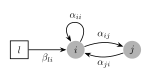
\includegraphics[width=0.8\textwidth]{modelli/modello influenza.pdf}
	\end{minipage}
	\begin{minipage}{0.5\textwidth}
		\begin{align*}
			l \;\; &\rightarrow \;\; \text{causa indipendente che influenza } i \\
			i,j  \;\; &\rightarrow \;\; \text{oggetti influenzati o influenzanti} \\
			\alpha, \beta\;\; &\rightarrow \;\; \text{parametri di influenza} \in \mathbb{R} 
		\end{align*}
	\end{minipage}
	\begin{align*}
		x_i(t/k) &\rightarrow \;\; \text{opinione del primo oggetto/persona, variabile di stato} \\
		x_j(t/k) &\rightarrow \;\; \text{opinione del secondo oggetto/persona, variabile di stato} \\
		\alpha_{ij} x_i(t/k) &\rightarrow \;\; \text{influenza di } i \text{ sull'oggetto } j \\
		\alpha_{ji} x_j(t/k) &\rightarrow \;\; \text{influenza di } j \text{ sull'oggetto } i \\
		\alpha_{ii} x_i(t/k) &\rightarrow \;\; \text{mantenimento della propria opinione} \\
		\beta_{li} u_l(t/k) &\rightarrow \;\; \text{influenza dall'ingresso indipendente } il \\
	\end{align*}
\end{center}

\subsubsection*{Rappresentazione in funzioni matematiche}
Per il tempo discreto si ottiene:
\[x_i(k+1) = \sum_{j=1}^{n} \alpha_{ji} x_j(k) + \sum_{l=1}^{p} \beta_{li} u_l(k) \qquad x(k+1) = Ax(k) + Bu(k) \quad a_{ij} = \alpha_{ji}\]
Per il tempo continuo si ottiene:
\[\dot{x}_i(t) = \sum_{j=1}^{n} \alpha_{ji} x_j(t) + \sum_{l=1}^{p} \beta_{li} u_l(t) \qquad \dot{x}(t) = Ax(t) + Bu(t) \quad a_{ij} = \alpha_{ji}\]
Esistono due modelli di influenza delle opinioni, per sistemi isolati, che hanno la particolarità di prevedere o meno l'influenza
dalle condizioni iniziali:
\begin{itemize}
	\item \textbf{modello di DeGroot}: lo stato non è influenzato dalla condizione iniziale e all'equilibrio tutti gli oggetti
	avranno la stessa opinione \[x(k+1) = \lambda A x(k) + (1-\lambda) \; x(0) \quad \lambda = 1 \quad \rightarrow \quad x(k+1) = A x(k)\]
	\item \textbf{modello di Friedkin e Johnsen}: lo stato è sempre influenzato dalla condizione iniziale e all'equilibrio le
	opinioni non convergono ad un consenso comune \[x(k+1) = \lambda A x(k) + (1-\lambda) \; x(0) \quad 0 \leq \lambda \leq 1\]
\end{itemize}

\newpage

\subsubsection*{Analisi qualitativa del diagramma delle fasi o spazio di stato}
Per risolvere i problemi di influenza si ricorre allo studio del diagramma delle fasi detto anche spazio di stato, ovvero del
grafico in cui, negli assi cartesiani sono presenti le variabili di stato e si è indipendenti dal tempo. Per semplicità si
scelgono solo modelli con due oggetti/persone e con ingressi costanti:
\begin{align*}
	&0 = \dot{x}_1(t) = \alpha_{11} x_1(t) + \alpha_{21} x_2(t) + \beta_{11} \bar{u}_1 + \beta_{21} \bar{u}_2 \\
	&0 = \dot{x}_2(t) = \alpha_{12} x_1(t) + \alpha_{22} x_2(t) + \beta_{12} \bar{u}_1 + \beta_{22} \bar{u}_2
\end{align*}
\begin{itemize}
	\item si analizzano le funzioni matematiche che descrivono il sistema all'equilibrio in maniera indipendente in modo da trovare
	delle equazioni che descrivono delle rette \(x_1 = m_1 x_2 + q_1\) e \(x_2 = m_2 x_1 + q_2\)
	\[x_1 = -\frac{\alpha_{21}}{\alpha_{11}} x_2 - \frac{\beta_{11} \bar{u}_1 + \beta_{21} \bar{u}_2}{\alpha_{11}} \qquad\qquad x_2 = -\frac{\alpha_{12}}{\alpha_{22}} x_1 - \frac{\beta_{12} \bar{u}_1 + \beta_{22} \bar{u}_2}{\alpha_{22}}\]
	\item si tracciano le rette nel diagramma delle fasi e si analizza il grafico ottenuto, se esiste il punto di equilibrio, allora
	è l'intersezione delle due rette
\end{itemize}

\subsubsection*{Esempi visti a lezione}
\begin{itemize}
	\item relazione amorosa tra Romeo e Giulietta
	\item corsa agli armamenti
	\item dinamica dei prezzi
\end{itemize}

\subsubsection*{Corsa agli armamenti a tempo continuo}
Sono presenti due nazioni che si influenzano a vicenda e due cause (aggressività delle nazioni) che influenzano rispettivamente
la prima e la seconda nazione.
\[\dot{x}_1(t) = -\alpha_{11} x_1(t) + \alpha_{21} x_2(t) + \bar{u}_1 \qquad x_1 = \frac{\alpha_{21}}{\alpha_{11}} x_2 + \frac{\bar{u}_1}{\alpha_{11}}\]
\[\dot{x}_2(t) = \alpha_{12} x_1(t) - \alpha_{22} x_2(t) + \bar{u}_2 \qquad x_2 = \frac{\alpha_{12}}{\alpha_{22}} x_1 + \frac{\bar{u}_2}{\alpha_{22}}\]

Per la corsa agli armamenti si era osservato che potevano verificarsi due casi, in base ai valori \(\alpha\):
\begin{itemize}
	\item[1.] le rette si incontrano nel punto di equilibrio e si divide il piano in 4 quadranti, analizzando i casi in cui \(\dot{x}_1(t) > 0\) e \(\dot{x}_2(t) > 0\)
	si osservava cosa avviene in ciascuno dei 4 quadranti: si tende all'equilibrio
	\item[2.] le rette non si incontrano e dividono il piano in 3 sezioni, analizzando cosa avveniva nelle tre sezioni si osserva che
	tra le due rette, il sistema diverge a \(+\infty\), altrimenti converge sulle due rette
\end{itemize}

\subsubsection*{Dinamica dei prezzi a tempo discreto}
Si definiscono i consumatori e i produttori con le loro sensibilità:
\[\begin{array}{l} q = b p + Q \\ q = -a p + D \end{array} \quad \begin{array}{l} p = \text{prezzo} \\ q = \text{quantità}\end{array} \quad \begin{array}{l} a = \text{sensib. consumatori} \\ b = \text{sensib. produttori}\end{array} \qquad \begin{array}{l} q(k) = -ap(k) + D \; \text{istantanea}\\ q(k\!+\!1) = bp(k) + Q \; \text{non istant.}\end{array}\]
Si analizza il grafico ottenuto dalle due rette in funzione dei parametri \(a, b\) e delle variabili di stato \(p, q\) e si
osserva che le rette sono sempre incidenti nel punto di equilibrio, ma si distinguono tre casi:
\begin{itemize}
	\item \(a > b\): scelto un punto sulle rette, si tende a convergere nell'intersezione attraverso moti oscillanti \say{rettangolari}
	esponenzialmente smorzati
	\item \(a = b\): scelto un punto sulle due rette, si ottiene un moto oscillante \say{rettangolare} costante, per cui non si
	raggiungerà mai l'equilibrio, a meno che non si parta proprio da esso
	\item \(a < b\): scelto un punto sulle due rette, si ottiene un moto oscillante \say{rettangolare} divergente, per cui non si
	raggiungerà mai l'equilibrio, a meno che non si parta proprio da esso
\end{itemize}
Tale analisi si ottiene analizzando il prezzo di equilibrio \(p_{eq} = -^1\!/\!_{(a+b)} \, (D-Q)\) e analizzando la deviazione del prezzo
rispetto all'equilibrio \(\tilde{p}(k+1) = -^b\!/\!_a \, \tilde{p(k)}\) con \(\tilde{p}(k) = p(k) - p_{eq}\).

\newpage


\subsection{Modelli fisici}
\subsubsection*{Circuiti elettrici}
Per modellare un circuito elettrico si utilizza un sistema matematico con i seguenti elementi:
\begin{itemize}
	\item \textbf{variabili di stato}: le tensioni dei condensatori e le correnti negli induttori
	\item \textbf{ingressi}: i vari generatori e disturbi
	\item \textbf{equazioni}: equazioni costitutive dei componenti e le leggi di Kirchhoff per il circuito
\end{itemize}

\subsubsection*{Sistemi meccanici traslazionali}
Per modellare i sistemi meccanici traslazionali (carrellino, molla, smorzatore) si definiscono:
\begin{itemize}
	\item \textbf{variabili di stato}: le posizioni e relative derivate dei carrellini/oggetti in movimento
	\item \textbf{ingressi}: le forze esterne agenti sul sistema
	\item \textbf{equazioni}: equazioni costitutive delle varie parti (molla, smorzatore), il primo principio della dinamica
	(inerzia) e il secondo principio (legge di Newton)
\end{itemize}

\subsubsection*{Sistemi meccanici rotativi}
Per modellare i sistemi meccanici rotativi (massa rotante, molla torsionale, smorzatore rotante) si definiscono:
\begin{itemize}
	\item \textbf{variabili di stato}: posizione angolare e relative derivate delle masse rotanti
	\item \textbf{ingressi}: momenti esterni agenti sul sistema
	\item \textbf{equazioni}: equazioni costitutive delle varie parti (molla torsionale e smorzatore torsionale), il primo
	principio della dinamica (inerzia) e il secondo principio (legge di Newton per rotazioni)
\end{itemize}

\subsection{Sistemi dinamici non lineari}
I sistemi fisici non lineari sono particolarmente ostici da analizzare dal punto vista matematico. Per cui, per studiarli, verranno
linearizzati attorno ai punti di equilibrio e ne verrà studiato il comportamento per brevi scostamenti dall'equilibrio.

\subsubsection*{Rappresentazione matematica di un sistema non lineare}
Il sistema non lineare non si può esprimere come combinazione lineare degli stati e degli ingressi/uscite, ma si utilizzano generiche
funzioni dipendenti dagli stati e dagli ingressi/uscite.
\begin{align*}
	&\text{tempo continuo} \quad \begin{cases} \dot{x}_1(t) = f_1 (x_1(t), \dots, x_n(t), u_1(t), \dots, u_m(t)) \\ \;\;\, \dots \; = \; \dots \\ \dot{x}_n(t) = f_n (x_1(t), \dots, x_n(t), u_1(t), \dots, u_m(t)) \end{cases} &\leftrightarrow \quad &\dot{x}(t) = f(x(t),u(t)) \\
	&\text{tempo discreto} \quad \begin{cases} x_1(k+1) = f_1 (x_1(k), \dots, x_n(k), u_1(k), \dots, u_m(k)) \\ \qquad\;\,\, \dots \; = \; \dots \\ x_n(k+1) = f_n (x_1(k), \dots, x_n(k), u_1(k), \dots, u_m(k)) \end{cases} &\leftrightarrow \quad &x(k+1) = f(x(k),u(k))
\end{align*}

\subsubsection*{Studio dell'equilibrio}
Si studiano le equazioni in modo da ottenere gli stati stazionari (tempo continuo) o i punti fissi (tempo discreto) tali per cui
si ha stabilità.
\begin{align*}
	&\text{tempo continuo} \quad \begin{cases} 0 = \dot{\bar{x}}_1(t) = f_1 (\bar{x}_1(t), \dots, \bar{x}_n(t), \bar{u}_1(t), \dots, \bar{u}_m(t)) \\ \qquad \dots \;\;\; = \;\;\; \dots \end{cases} \\
	&\text{tempo discreto} \quad \begin{cases} \bar{x}_1(k) = f_1 (\bar{x}_1(k), \dots, \bar{x}_n(k), \bar{u}_1(k), \dots, \bar{u}_m(k)) \\ \;\;\:\, \dots \; = \; \dots  \end{cases}
\end{align*}

\subsubsection*{Linearizzazione all'equilibrio}
Attraverso l'espansione di Taylor si linearizzano le funzioni intorno ai punti di equilibrio con:
\begin{itemize}
	\item \((\bar{x}_{eq},\bar{u}_{eq}) = (\bar{x}_1, \dots \bar{x}_n, \bar{u}_1, \dots, \bar{u}_m)\)
	\item \((\tilde{x},\tilde{u}) = (x,u)-(x_{eq},u_{eq}) \;\; \rightarrow \;\; (\tilde{x}_{eq},\tilde{u}_{eq}) = (\vec{0},\vec{0})\)
\end{itemize}

\vspace{10pt}
\noindent
Di seguito la linearizzazione di \(f_1\) in tempo continuo con Taylor, si osserva che si ottiene una combinazione lineare delle
variabili di stato e degli ingressi in cui i coefficienti sono ottenuti dalle derivate parziali.
\begin{align*}
	\dot{x}_1(t) &= f_1(x_1(t), \dots x_n(t), u_1(t), \dots, u_m(t)) = \\
	\dot{x}_1(t) &\approx \underbrace{f_1(\bar{x}_1, \dots \bar{x}_n, \bar{u}_1, \dots, \bar{u}_m)}_{=0} + \underbrace{ \left. \frac{\partial f_1}{\partial x_1} \right|_{\bar{x}, \bar{u}} }_{{a_{11}}} \underbrace{ \left( x_1(t) - \bar{x}_1 \right) }_{\tilde{x}_1} + \cdots + \underbrace{ \left. \frac{\partial f_1}{\partial x_n} \right|_{\bar{x}, \bar{u}} }_{a_{1n}} \underbrace{ \left( x_n(t) - \bar{x}_n \right) }_{\tilde{x}_n} + \\
	&\qquad\qquad\qquad\qquad\qquad\qquad + \underbrace{ \left. \frac{\partial f_1}{\partial u_1} \right|_{\bar{x}, \bar{u}} }_{{b_{11}}} \underbrace{ \left( u_1(t) - \bar{u}_1 \right) }_{\tilde{u}_1} + \cdots + \underbrace{ \left. \frac{\partial f_1}{\partial u_m} \right|_{\bar{x}, \bar{u}} }_{b_{1m}} \underbrace{ \left( u_m(t) - \bar{u}_m \right) }_{\tilde{u}_m} \\
	\dot{x}_1(t) &\approx a_{11} \tilde{x}_1 + \dots + a_{1n} \tilde{x}_n + b_{11} \tilde{u}_1 + \dots + b_{1m} \tilde{u}_m
\end{align*}

\[\text{In generale} \qquad \dot{\tilde{x}}(t) \approx A \tilde{x}(t) + B \tilde{u}(t) \qquad\qquad A = (a_{ij}) \quad a_{ij} = \left. \frac{\partial f_i}{\partial x_j} \right|_{\bar{x}, \bar{u}} \qquad B = (b_{ij}) \quad b_{ij} = \left. \frac{\partial f_i}{\partial u_j} \right|_{\bar{x}, \bar{u}}\]

\vspace{10pt}
\noindent
Di seguito la linearizzazione di \(f_1\) in tempo discreto con Taylor, si osserva che si ottiene una combinazione lineare delle
variabili di stato e degli ingressi in cui i coefficienti sono ottenuti dalle derivate parziali.
\begin{align*}
	x_1(k+1) &= f_1(x_1(k), \dots x_n(k), u_1(k), \dots, u_m(k)) = \\
	x_1(k+1) &\approx \underbrace{f_1(\bar{x}_1, \dots \bar{x}_n, \bar{u}_1, \dots, \bar{u}_m)}_{=0} + \underbrace{ \left. \frac{\partial f_1}{\partial x_1} \right|_{\bar{x}, \bar{u}} }_{{a_{11}}} \underbrace{ \left( x_1(k) - \bar{x}_1 \right) }_{\tilde{x}_1} + \cdots + \underbrace{ \left. \frac{\partial f_1}{\partial x_n} \right|_{\bar{x}, \bar{u}} }_{a_{1n}} \underbrace{ \left( x_n(k) - \bar{x}_n \right) }_{\tilde{x}_n} + \\
	&\qquad\qquad\qquad\qquad\qquad\qquad + \underbrace{ \left. \frac{\partial f_1}{\partial u_1} \right|_{\bar{x}, \bar{u}} }_{{b_{11}}} \underbrace{ \left( u_1(k) - \bar{u}_1 \right) }_{\tilde{u}_1} + \cdots + \underbrace{ \left. \frac{\partial f_1}{\partial u_m} \right|_{\bar{x}, \bar{u}} }_{b_{1m}} \underbrace{ \left( u_m(k) - \bar{u}_m \right) }_{\tilde{u}_m} \\
	x_1(k+1) &\approx a_{11} \tilde{x}_1 + \dots + a_{1n} \tilde{x}_n + b_{11} \tilde{u}_1 + \dots + b_{1m} \tilde{u}_m
\end{align*}

\[\text{In generale} \qquad \tilde{x}(k+1) \approx A \tilde{x}(k) + B \tilde{u}(k) \qquad\quad A = (a_{ij}) \quad a_{ij} = \left. \frac{\partial f_i}{\partial x_j} \right|_{\bar{x}, \bar{u}} \qquad B = (b_{ij}) \quad b_{ij} = \left. \frac{\partial f_i}{\partial u_j} \right|_{\bar{x}, \bar{u}}\]

\section{Analisi a tempo continuo}
\subsection{Sistemi lineari a tempo invariante - LTI}
\subsubsection*{Assunzioni}
Un sistema di dice lineare a tempo invariante (LTI) se:
\begin{itemize}
	\item i coefficienti non cambiano nel tempo
	\item vale il principio di sovrapposizione degli effetti
	\item si ha invarianza nel tempo, ovvero se a partire dalle stesse condizioni una certa causa \(u(t)\) ha sempre lo stesso
	effetto \(x(t)\) anche se viene ritardata \(u(t-t_0)\) di un tempo \(t_0\)
\end{itemize}

\subsubsection*{Sovrapposizione degli effetti}
Per il principio di sovrapposizione degli effetti, dato un sistema LTI \(\dot{x}(t) = Ax(t) + Bu(t)\):
\begin{itemize}
	\item se \(x'(t)\) è soluzione per le condizioni iniziali \(x'(0)\) e ingressi \(u'(t)\)
	\item se \(x''(t)\) è soluzione per le condizioni iniziali \(x''(0)\) e ingressi \(u''(t)\)
	\item se \(x'''(0) = \alpha x'(0) + \beta x''(0)\) e \(u'''(t) = \alpha u'(t) + u''(t)\)
	\[\text{allora si ottiene una nuova soluzione: } \qquad x'''(t) = \alpha x'(t) + x''(t)\]
\end{itemize}
Ciò significa che se si è in grado di scomporre le condizioni iniziali e gli ingressi in due parti \(x'(0),u'(t)\), \(x''(0),u''(t)\)
e si conoscono le soluzioni \(x'(t),x''(t)\) per i due sottoproblemi allora per trovare la soluzione completa è sufficiente
sommare le due soluzioni parziali.

\subsubsection*{Introduzione all'evoluzione libera e alla risposta forzata}
Si definiscono quindi due situazioni per cui risulta più facile calcolare le soluzioni:
\begin{itemize}
	\item \textbf{evoluzione libera}: con condizioni iniziali non nulle \(x(0) \neq 0\) e  ingressi nulli \(u(t) = 0\)
	\item \textbf{risposta forzata}: con condizioni iniziali nulle \(x(0) = 0\) e ingressi non nulli \(u(t) \neq 0\)
\end{itemize}
La soluzione generale del sistema con condizioni iniziali \(x(0)\) dell'evoluzione libera e con ingressi \(u(t)\) della risposta
forzata sarà data dalla somma della soluzione dell'evoluzione libera con quella della risposta forzata.

\newpage

\subsection{Evoluzione libera}
\subsubsection*{Introduzione}
L'evoluzione libera \(x_l(t)\) di un sistema LTI \(\dot{x}(t) = Ax(t) + Bu(t)\) è la soluzione parziale del sistema ottenuta
considerando solo le condizioni iniziali \(x(0) \neq 0\), ponendo gli ingressi a zero \(u(t) = 0\).

\subsubsection*{Calcolo dell'evoluzione libera}
Dato un sistema LTI \(\dot{x}(t) = Ax(t) + Bu(t)\) di cui si vuole analizzare l'evoluzione libera:
\begin{itemize}
	\item[1.] si pongono gli ingressi a zero \(u(t) = 0\) e si scelgono determinate condizioni iniziali \(x(0) \neq 0\), per
	cui l'equazione del sistema diventa \[\dot{x}(t) = Ax(t)\]
	\item[2.] è possibile esprimere il vettore \(x(t)\) come combinazione lineare degli autovettori di \(A\) ottenendo \(x(t) = c_1 v_1 + c_2 v_2 + \dots\)
	per cui l'equazione diventa \[\dot{x}(t) = A(c_i v_1 + c_2 v_2 + \dots)\]
	\item[3.] per la proprietà degli autovettori \(A v_i = \lambda_i v_i\), con \(\lambda_i\) autovalore associato, l'equazione
	diventa \[\dot{x}(t) = Ax(t) = c_1 \lambda_1 v_1 + c_2 \lambda_2 v_2 + \dots\]
	\item[4.] per linearità del sistema si studia ogni contributo indipendentemente e alla fine si sommano tutti i risultati
	ottenuti, la soluzione di un generico contributo (si pone \(x(t) = c_i v_i\)) vale
	\[\dot{x}(t) = c_i \lambda_i v_i \;\; \Leftrightarrow \;\; x_{l,i}(t) = c_i e^{\lambda_i t} v_i \;\; (= x_0 e^{\lambda_i t})\]
	\item[5.] dalla somma di tutti i contributi si ottiene la soluzione dell'evoluzione libera
	\[x_l(t) = \sum_{i=1}^{n} c_i e^{\lambda_i t} v_i \qquad \qquad \text{con } x(0) = \sum_{i=0}^{n} c_i v_i, \quad \begin{array}{l}
		\lambda_i, v_i = \text{autovalori e autovettori di } A \\
		e^{\lambda_i t} v_i =  \text{modo naturale associato a } \lambda_i
	\end{array}\]
\end{itemize}

\subsubsection*{Modi naturali reali}
Dato il modo naturale \(e^{\lambda_i t} v_i\) relativo all'autovalore \(\lambda_i\), se \(\lambda_i \in \mathbb{R}\), il modo
naturale viene detto reale e:
\begin{center}
	\begin{minipage}{0.5\textwidth}
		\begin{itemize}
			\item come traiettoria evolutiva nel diagramma delle fasi ha una retta che passa per il punto \(x(t)\) e ha come vettore
			direttore proprio l'autovettore del modo naturale reale
			\item come evoluzione nel tempo ha un andamento esponenziale che dipende da \(\lambda_i\):
			\begin{itemize}
				\item se \(\lambda_i > 0\) moto esponenziale divergente
				\item se \(\lambda_i = 0\) moto costante 
				\item se \(\lambda_i < 0\) moto esponenziale convergente
			\end{itemize}
			\item ha costante di tempo caratteristica del modo naturale reale: \(\displaystyle\tau_i = -\frac{1}{\lambda_i}\)
		\end{itemize}
	\end{minipage}
	\begin{minipage}{0.49\textwidth}
		\centering
		\includegraphics[width=0.8\textwidth]{immagini/evoluzione libera reale 1.png}
		\includegraphics[width=0.8\textwidth]{immagini/evoluzione libera reale 2.png}
	\end{minipage}
\end{center}
In conclusione l’evoluzione libera è la combinazione lineare di \(n\) modi naturali a cui corrispondono \(n\) traiettorie,
ciascuna delle quali evolve lungo il sottospazio unidimensionale determinato dal corrispondente autovettore \(v_i\).

\newpage

\subsubsection*{Modi naturali complessi}
Se dalla soluzione \(x_l(t)\) si ottengono due autovalori \(\lambda_{k1}, \lambda_{k2}\) complessi coniugati tali che
\(\lambda_{k1,k2} = \sigma_k \pm j\omega_k\) allora si avrà anche degli autovettore complessi coniugati \(v_{k1,k2} = v_{ka} \pm j v_{kb}\).
Il modo naturale complesso associato sarà della forma:
\[x(t) = m_k e^{\sigma_k t} \; [ \sin(\omega_k t + \varphi_k) v_{ka} + \cos (\omega_k t + \varphi_k) v_{kb}]\]
\[\text{con}\quad m_p = \sqrt{{c_{ka}}^2 + {c_{kb}}^2} \qquad x(0) = c_{ka} v_{ka} + c_{kb} v_{kb} \qquad
\varphi = \begin{cases} \arctan (c_{ka} / c_{kb}) & c_{kb} > 0 \\ \arctan (c_{ka} / c_{kb}) + \pi & c_{kb} < 0 \end{cases}\]
Analizzando il modo naturale complesso si osserva che:
\begin{center}
	\begin{minipage}{0.5\textwidth}
		\begin{itemize}
			\item come traiettoria evolutiva nel diagramma delle fasi ha una spirale ellittica che parte per il punto \(x(t)\)
			e che può convergere, divergere o rimanere costante in funzione di \(\sigma_k\)
			\item come evoluzione nel tempo ha un andamento esponenziale oscillatorio che dipende da \(\sigma_k\):
			\begin{itemize}
				\item se \(\sigma_k > 0\) moto oscillante divergente
				\item se \(\sigma_k = 0\) moto periodico 
				\item se \(\sigma_k < 0\) moto oscillante convergente
			\end{itemize}
			\item ha costante di tempo caratteristica del modo naturale complesso : \(\displaystyle\tau_k = -\frac{1}{\sigma_k}\)
		\end{itemize}
	\end{minipage}
	\begin{minipage}{0.49\textwidth}
		\centering
		\includegraphics[width=0.8\textwidth]{immagini/evoluzione libera complessa 1.png}
		\vspace{10pt}
		
		\includegraphics[width=0.9\textwidth]{immagini/evoluzione libera complessa 2.png}
	\end{minipage}
\end{center}

\subsubsection*{Evoluzione libera completa: modi naturali reali + complessi}
Mettendo insieme l'evoluzione libera costituita dai moti naturali reali e quella costituita dai moti naturali complessi si ottiene
la formula generale dell'evoluzione libera (considerando che \(A\) abbia \(n\) autovalori distinti):
\[x_l(t) = \sum_{i=1}^{\mu} c_i e^{\lambda_i t} v_i + \sum_{k=1}^{\nu} m_k e^{\sigma_k t} [ \sin(\omega_k t + \varphi_k) v_{ka} + \cos (\omega_k t + \varphi_k) v_{kb}]\]
\[\text{con} \qquad x(0) = \sum_{i=1}^{\mu} c_i v_i + \sum_{k=1}^{\nu} c_{ka} v_{ka} + c_{kb} v_{kb} \qquad n = \mu + 2\nu\]
In base al posizionamento degli autovalori nel piano complesso si hanno diversi moti evolutivi del sistema:
\begin{center}
	\includegraphics[width=0.6\textwidth]{immagini/evoluzione libera generale.png}
\end{center}

\subsubsection*{Evoluzione libera come esponenziale di una matrice}
L'esponenziale di una matrice è definito sfruttando lo sviluppo di Taylor dell'esponenziale nell'origine
\[e^A = \sum_{i=0}^{+\infty} \frac{A^k}{k!} = I + A + \frac{A^2}{2} + \dots\]
Si dimostra che l'espressione dell'evoluzione libera corrisponde all'esponenziale della matrice \(A\)
\[x_l(t) = \sum_{i=1}^{n} c_i e^{\lambda_i t} v_i = e^{At} x(0) \qquad \qquad \text{con} \;\; x(0) = \sum_{i=1}^{n} c_i v_i\]

\subsection{Risposta forzata}
\subsubsection*{Introduzione}
La risposta forzata \(x_f(t)\) di un sistema LTI \(\dot{x}(t) = Ax(t) + Bu(t)\) è la soluzione parziale del sistema ottenuta
considerando l'evoluzione del sistema di fronte agli ingressi non nulli \(u(t) \neq 0\), ponendo le condizioni
iniziali a zero \(x(0) = 0\).

\subsubsection*{Calcolo della risposta forzata}
Dato un sistema LTI \(\dot{x}(t) = Ax(t) + Bu(t)\) di cui si vuole analizzare la risposta forzata:
\begin{itemize}
	\item[1.] si pongono le condizioni iniziali a zero \(x(0) = 0\) e si analizza il sistema in funzione degli ingressi
	\(u(t) \neq 0\), per cui l'equazione del sistema rimane \[\dot{x}(t) = Ax(t) + Bu(t) \qquad \text{con} \quad x(0) = 0\]
	\item[2.] risolvendo l'equazione differenziale si ottiene che la formula per la risposta forzata vale
	\[x_f(t) = \int_{0}^{t} e^{A(t-\tau)} Bu(\tau) d\tau\]
	\item[3.] analizzando per un certo ingresso fissato \(u(t) = \bar{u}\) e ponendo \(\xi = (t - \tau)\) si ha:
	\[x_f(t) = \int_{0}^{t} e^{A(t-\tau)} Bu(\tau) d\tau = \int_{t}^{0} e^{A\xi} B\bar{u} -d\xi = \left(\int_{0}^{t} e^{A\xi} B d\xi\right) \bar{u}\]
	\item[4.] se la matrice \(A\) è invertibile si ottiene
	\[\int_{0}^{t} e^{A\xi} B d\xi = \left. A^{-1} e^{A\xi} B \right|_0^t = A^{-1} \left(e^{A\xi} - I\right) B \quad \rightarrow \quad x_f(t) = A^{-1} \left(e^{A\xi} - I\right) B \bar{u}\]
	\item[5.] se la matrice \(A\) non è invertibile si usa sovrapposizione degli effetti per ogni ingresso \(1, \dots, m\) (colonne
	della matrice \(B\)) e sarà necessario calcolare l'integrale, in caso è possibile notare che la risposta forzata corrisponde 
	all'evoluzione libera con condizioni iniziali \(B_i\)
	\[x_f(t) = \sum_{i=1}^{m} \left(\int_{0}^{t} e^{A\xi} B_i d\xi\right) \bar{u}_i = \sum_{i=1}^{m} \left(\int_{0}^{t} \left.x_l(t) \right|_{x(0)=B_i} d\xi\right) \bar{u}_i = \sum_{i=1}^{m} \left(\int_{0}^{t} \sum_{j=1}^{n} \left(c_j e^{\lambda_j t} v_j\right)  d\xi\right) \bar{u}_i\]
	\[\text{con} \qquad B_i = \sum_{j=1}^{n} c_j v_j\]
\end{itemize}

\newpage


\subsection{Convoluzione}
\subsubsection*{Risposta impulsiva}
La risposta impulsiva è una funzione matematica che descrive la risposta forzata di un sistema perturbato da un impulso unitario,
ovvero quando \(u(t) = \delta(t)\):
\[h(t) := e^{At}B \qquad\qquad \left. x_f(t) \right|_{u(t) = \delta(t)} = \int_{0}^{t} h(t-\tau) \, \delta(t) \, d\tau= h(t)\]

\subsubsection*{Risposta forzata come prodotto di convoluzione}
La risposta forzata può essere interpretata come un integrale della convoluzione (o prodotto di convoluzione), ovvero la
combinazione tra risposta impulsiva \(h(t)\) e l'ingresso \(u(t)\):
\[x_f(t) = (h * u)(t) := \int_{-\infty}^{+\infty} h(t - \tau) u(\tau) \, d\tau\]

\begin{itemize}
	\item l'impulso di Dirac è l'elemento neutro del prodotto di convoluzione \(x_f(t) = (h * \delta)(t) = h(t)\)
	\item poiché la risposta di un sistema LTI a un impulso di Dirac è la risposta impulsiva \(h(t)\), la risposta forzata a un
	ingresso \(u(t)\) è la somma pesata (tramite \(u(t)\)) delle risposte impulsive \(h(t)\) traslate nel tempo.
\end{itemize}

\subsection{Trasformata di Laplace}
\subsubsection*{Definizione}
La trasformata di Laplace mappa funzioni nel dominio del tempo in funzioni nel dominio dei numeri complessi permettendo di
semplificare i calcoli di analisi dei sistemi.
\[\lap : f \left(\begin{array}{l} \mathbb{R} \to \mathbb{R} \\ t \mapsto f(t) \end{array}\right) \mapsto F \left(\begin{array}{l} \mathbb{C} \to \mathbb{C} \\ s \mapsto F(s) \end{array}\right) \qquad F(s) = \lap[f(t)] := \int_{0^-}^{+\infty} f(t) e^{st} dt\]

\subsubsection*{Osservazioni}
\begin{itemize}
	\item si considera solo la trasformata di Laplace unilatera (solo per tempi positivi o nulli)
	\item il fattore \(e^{st}\) serve per far convergere l'integrale a \(t \to +\infty\)
	\item per rendere l'esponente \(st\) adimensionale, \(s\) ha dimensioni di una frequenza
	\item siccome è un integrale indefinito, l'integrale va trattato con un limite
	\item l'integrale non dipende da \(t\), ma solo dal parametro \(s\), per questo \(F\) dipende solo da \(s\)
	\item se l'integrale converge per un certo valore \(s_0\), allora convergerà per tutti i valori \(\Real(s) > \Real(s_0)\), si 
	definisce, quindi, l'ascissa di convergenza \(\sigma_c\) che separa il semipiano sinistro con \(s\) convergenti da quello
	destro con \(s\) convergenti
\end{itemize}

\subsubsection*{Proprietà}
\begin{itemize}
	\item unicità: se esiste la trasformata è unica e vale \(\lap[f(t)] = F(s) \qquad \lap^{-1}[F(s)] = f(t)\)
	\item linearità: \(\lap[\alpha f(t) + \beta g(t)] = \alpha\lap[f(t)] + \beta\lap[g(t)] = \alpha L(s) + \beta G(s)\)
	\item proprietà della derivata e dell'integrale: \(\lap\left[\frac{d f(t)}{dt}\right] = sF(s) - f(0^-) \qquad \lap\left[\int_0^t f(t) dt \right] = F(s)/s\)
	\item convoluzione: \(\lap[(f*h)(t)] = F(s)H(s)\)
	\item traslazione temporale: \(\lap[f(t-a)] = e^{-as} F(s)\)
	\item traslazione in frequenza: \(\lap[e^{at}f(t)] = F(s-a)\)
	\item teorema del valore iniziale: \(\displaystyle \lim_{t \to 0^+} f(t) = \lim_{s \to +\infty} sF(s)\)
	\item teorema del valore finale: \(\displaystyle \lim_{t \to +\infty} f(t) = \lim_{s \to 0} sF(s)\)
\end{itemize}

\subsubsection*{Tabelle per trasformata e antitrasformata}
\begin{center}
	\begin{tabularx}{\textwidth}{ C | C }
		\textbf{Funzione del tempo} & \textbf{Trasformata di Laplace} \\
		\toprule
		\(\delta(t)\) (impulso di Dirac) & 1 \\
		\midrule
		\(\delta_{-1}(t)\) (gradino unitario) & \(1/s\) \\
		\midrule
		\(\delta_{-2}(t)\) (rampa unitaria) & \(1/s^2\) \\
		\midrule
		\(e^{at}\) (esponenziale) & \(\dfrac{1}{s - a}\) \\
		\midrule
		\(\dfrac{t^{n-1}}{(n-1)!} e^{at}\) (esponenziale polinomiale) & \(\dfrac{1}{(s - a)^n}\) \\
		\midrule
		\(\sin(\omega t)\) (sinusoide) & \(\dfrac{\omega}{s^2 + \omega^2}\) \\
		\midrule
		\(\cos(\omega t)\) (cosinusoide) & \(\dfrac{s}{s^2 + \omega^2}\) \\
		\midrule
		\(\dfrac{1}{\omega_n \sqrt{1 - \zeta^2}} e^{-\zeta \omega_n t} \sin\big(\omega_n \sqrt{1 - \zeta^2} t \big)\) & 
		\(\dfrac{1}{s^2 + 2\zeta \omega_n s + \omega_n^2}\) (fattore trinomio) \\
		\midrule
		\(e^{-at} \cos(\omega t)\) & \(\dfrac{s + a}{(s + a)^2 + \omega^2}\) \\
		\midrule
		\(e^{-at} \sin(\omega t)\) & \(\dfrac{\omega}{(s + a)^2 + \omega^2}\)
	\end{tabularx}
\end{center}

\subsubsection*{Antitrasformata}
Definita la trasformata di Laplace come sopra, l'antitrasformata è definita come segue:
\[\lap[f(t)] = \int_{0^-}^{+\infty} f(t) e^{-st} dt \qquad\qquad \lap^{-1}[F(s)] = \frac{1}{2\pi j} \int_{\sigma-j\infty}^{\sigma+j\infty} F(s) e^{st} ds \qquad \text{con} \; \sigma > \sigma_c\]
Siccome l'integrale dell'antitrasformata è ostico da calcolare, si ricorre all'uso della tabella sopra. Di solito le funzioni
da antitrasformare sono un rapporto tra polinomi in \(s\) per cui si definiscono alcune regole e procedimenti ricondursi alle
forme in tabella:
\begin{itemize}
	\item[1.] si scrive la funzione come rapporto di polinomi \(\mathcal{N}(s)\) e \(\mathcal{D}(s)\)
	\item[2.] si scompone il denominatore esplicitandone le radici (reali o complesse), dette poli
\end{itemize}
\[F(s) = \frac{\mathcal{N}(s)}{\mathcal{D}(s)} = \frac{\mathcal{N}(s)}{(s-\lambda_1)^{\mu_1}(s-\lambda_2)^{\mu_2}\dots(s-\lambda_n)^{\mu_n}} = \dots\]

\subsubsection*{Antitrasformata per poli semplici}
\begin{itemize}
	\item[3.] se i poli hanno molteplicità unitaria, si può dividere la frazione in fratti semplici \(C_i \; / \; (s-\lambda_i)\)
	\[\dots = \frac{C_1}{s-\lambda_1} + \frac{C_2}{s-\lambda_2} + \dots + \frac{C_n}{s-\lambda_n} \qquad \text{con} \qquad C_i = \lim_{s \to \lambda_i} (s-\lambda_i) F(s)\]
	\item[4.] si antitrasformano i fratti semplici individualmente, in caso di poli reali le soluzioni sono esponenziali, in
	caso di poli complessi coniugati, le soluzioni si combinano ottenendo moti oscillatori
	\[\lap^{-1}\left[\frac{C_i}{s-\lambda_i}\right] = C_i e^{\lambda_i t} \qquad\quad C_i e^{\lambda_i t} + {C_i}^* e^{{\lambda_i}^* t} = 2e^{\sigma t} (a \cos(\omega t) - b \sin(\omega t)) \quad \begin{array}{l} C,C^* = a \pm jb \\[5pt] \lambda,\lambda^* = \sigma \pm j\omega \end{array}\]
\end{itemize}

\newpage

\subsubsection*{Antitrasformata per poli multipli}
\begin{itemize}
	\item[3.] se i poli hanno molteplicità maggiore di 1, si considera un residuo per ogni esponente da 1 a \(\mu_i\)
	\[\dots = \dots \frac{C_{i,0}}{(s-\lambda_i)} + \frac{C_{i,1}}{(s-\lambda_i)^2} + \dots + \frac{C_{i,\mu_i-1}}{(s-\lambda_i)^{\mu_i}} + \dots\]
	\begin{align*}
		C_{i,\mu_i-1} &= \lim_{s \to \lambda_i} F(s) (s-\lambda_i)^{\mu_i} &\qquad C_{i,\mu_i-2} &= \lim_{s \to \lambda_i} \left(F(s) - \frac{C_{i,\mu_i-1}}{(s-\lambda_i)^{\mu_i}} \right) (s-\lambda_i)^{\mu_i-1} \\
		\quad &\dots\quad  &\qquad C_{i,0} &= \lim_{s \to \lambda_i} \left(F(s) - \sum_{l=1}^{\mu_i-1} \frac{C_{i,l}}{(s-\lambda_i)^{l+1}} \right) (s-\lambda_i)
	\end{align*}
	\item[4.] si antitrasformano i fratti raggruppando quelli associati ad uno stesso autovalore:
	\[\lap^{-1}\left[ \sum_{l=0}^{\mu_i-1} \frac{C_{i,l}}{(s-\lambda_i)^{l+1}} \right] = \sum_{l=0}^{\mu_i-1} C_{i,l} \frac{t^l}{l!} e^{\lambda_i t}\]
\end{itemize}

\subsubsection*{Moti naturali di poli semplici}
\begin{center}
	\includegraphics[width=0.9\textwidth]{immagini/laplace poli semplici.png}
\end{center}

\subsubsection*{Moti naturali di poli multipli}
\begin{center}
	\includegraphics[width=0.9\textwidth]{immagini/laplace poli multipli.png}
\end{center}

\subsubsection*{Evoluzione libera con Laplace}
Studio dell'evoluzione libera attraverso la trasformata di Laplace
\[\dot{x}_l(t) = Ax_l(t) \;\;\stackrel{\lap}{\longrightarrow}\;\; sX_l(s) - x_l(0) = AX_l(s) \;\;\rightarrow\;\; sX_l(s)-AX_l(s) = x_l(0) \;\;\rightarrow\;\; (sI-A)X_l(s) = x_l(0)\]
\[(sI-A)X_l(s) = x_l(0) \;\;\rightarrow\;\; X_l(s) = (sI-A)^{-1} x_l(0) \;\;\stackrel{\lap^{-1}}{\longrightarrow}\;\; x_l(t) = e^{At} x_l(0)\]

\subsubsection*{Risposta forzata con Laplace}
Studio della risposta forzata attraverso la trasformata di Laplace
\[\dot{x}_f(t) = Ax_f(t) + Bu(t) \;\;\stackrel{\lap}{\longrightarrow}\;\; sX_f(s) - x_f(0) = AX_f(s) + BU(s) \;\;\rightarrow\;\; X_f(s) = (sI-A)^{-1}BU(s)\]
Si definisce la matrice di trasferimento tra ingressi e stato, che è anche la risposta impulsiva del sistema:
\[\frac{X_f(s)}{U(s)} = (sI-A)^{-1}B \qquad\qquad X_f(s) = H(s)U(s) \;\;\rightarrow\;\; \frac{X_f(s)}{U(s)} = H(s) = (sI-A)^{-1}B\]
Se si definiscono le uscite del sistema come \(y(t) = Cx(t) + Du(t)\), allora è possibile definire la matrice di trasferimento tra 
ingressi e uscite: \[\frac{Y(s)}{U(s)} = C(sI-A)^{-1}B + D\]

\subsubsection*{Risposta complessiva (libera + forzata) con Laplace}
Unendo l'evoluzione libera e la risposta forzata trasformate con Laplace si ottiene:
\[X(s) = X_l(s) + X_f(s) = (sI-A)^{-1} x_l(0) + (sI-A)^{-1}BU(s)\]

\subsection{Risposta in frequenza}
\subsubsection*{Risposta in frequenza in un sistema BIBO stabile}
L'analisi della risposta in frequenza consiste nell'analizzare come varia l'ampiezza e la fase tra un segnale in ingresso e un segnale
in uscita di un sistema BIBO-stabile. Si considerano solo sistemi BIBO-stabili in quanto, se perturbati con un segnale sinusoidale ad
una certa frequenza, restituiscono sempre un segnale sinusoidale alla stessa frequenza alterato di ampiezza e fase.

\subsubsection*{Analisi in frequenza e diagrammi di Bode}
Per l'analisi in frequenza si eseguono i seguenti passaggi:
\begin{itemize}
	\item[1.] si calcola la sola risposta forzata di un sistema BIBO stabile e si ottiene la risposta impulsiva del sistema trasformata
	con Laplace (o funzione di trasferimento): \(H(s) = X_f(s) / U(s)\)
	\item[2.] si studia la risposta in frequenza (in uscita) del sistema perturbato da una sinusoide (in ingresso) analizzando come
	varia l'ampiezza e la fase in funzione di \(\omega\):
	\[x_r(t) := \left|H(j\omega)\right| \sin (\omega t + \arg{\left\{H(j\omega)\right\}}) \qquad \text{ampiezza} = \left|H(j\omega)\right| \qquad \text{fase} = \arg{\left\{H(j\omega)\right\}}\]
	\item[3.] è possibile disegnare i grafici che si ottengono studiando ampiezza e fase in funzione della frequenza che prendono il
	nome di diagrammi di Bode; ampiezza \((20\log_{10}(H(j\omega)) = [dB])\) e frequenza \((\log_{10}(\omega))\) sono indicate in
	scala logaritmica per una migliore lettura
\end{itemize}

\subsubsection*{Frequenza o pulsazione di taglio}
Nel caso di sistemi BIBO che fungono da filtri (abbassano l'ampiezza di frequenze sopra o sotto una certa soglia) si definisce la
pulsazione di taglio quando la parte reale uguaglia la parte immaginaria e si ha un'attenuazione dell'ampiezza di \(-3 \; \text{dB}\)
o \(70\%\) e la fase si inverte di \(\pi/4\):
\[\left. H(j\omega) \right|_{\omega = \omega_\text{taglio}} = \frac{\sqrt{2}}{2} = 0.7 \qquad\qquad 20\log_{10}\left(\left. H(j\omega) \right|_{\omega = \omega_\text{taglio}}\right) = -3 \; \text{dB}\]

\newpage


\section{Analisi a tempo discreto}
\subsection{Parallelismo tra tempo continuo e tempo discreto}
\begin{center}
	\begin{tabularx}{\textwidth}{l | C | C}
		& \textbf{tempo continuo} & \textbf{tempo discreto} \\
		\toprule
		\multirow{2}{*}{equazioni} & \(\dot{x}(t) = Ax(t) + Bu(t)\) & \(x(k+1) = Ax(k) + Bu(k)\) \\
		& \(x(t) = x_l(t) + x_f(t)\) & \(x(k) = x_l(k) + x_f(k)\) \\
		\midrule
		condizioni iniziali & \(x_0 = c_1 v_1 + \dots + c_n v_n\) & \(x_0 = c_1 v_1 + \dots + c_n v_n\) \\
		\midrule
		modo naturale & \(e^{\lambda_i t} v_i\) & \({\lambda_i}^k v_i\) \\
		\midrule
		evoluzione & \(\lambda_i < 0\) convergente, \(\lambda_i = 0\) costante, \(\lambda_i > 0\) divergente & \(\left|\lambda_i\right| < 1\) convergente, \(\left|\lambda_i\right| = 1\) costante, \(\left|\lambda_i\right| > 1\) divergente, \(\lambda_i < 0\) alternati \\
		\midrule
		evoluzione libera & \(x_l(t) = \sum_{i=1}^{n} c_i e^{\lambda_i t} v_i = e^{At} x_0\) & \(x_l(k) = \sum_{i=1}^{n} c_i {\lambda_i}^k v_i = A^k x_0\) \\
		\midrule
		\multirow{3}{*}{risposta forzata} & \(x_f(t) = \int_{0}^{t} e^{A(t-\tau)}Bu(\tau) d\tau\) & \(x_f(k) = \sum_{h=0}^{k-1} A^{k-h-1} B u(h)\) \\
		& \(x_f(t) = \left(\int_{0}^{t} e^{A\xi}B d\xi\right) \bar{u}\) & \(x_f(t) = \left(\sum_{\xi=0}^{k-1} A^\xi B\right) \bar{u}\) \\
		& \(x_f(t) = \sum_{i=1}^{p} \left(\int_{0}^{t} e^{A\xi}[B]_i d\xi\right) \bar{u}_i\) & \(x_f(t) = \sum_{i=1}^{p} \left(\sum_{\xi=0}^{k-1} A^\xi [B]_i\right) \bar{u}_i\) \\
		\bottomrule
	\end{tabularx}
\end{center}

\subsubsection*{Andamenti delle evoluzioni (convergenti, divergenti, oscillanti, alterni)}
\begin{center}
	\begin{tabularx}{\textwidth}{C C}
		\midrule
		diagramma delle fasi in tempo continuo & diagramma delle fasi in tempo discreto
	\end{tabularx}
	\includegraphics[width=\textwidth]{immagini/tempo discreto 1.png}
	\vspace{10pt}

	\begin{tabularx}{\textwidth}{C C}
		\midrule
		modi naturali in tempo continuo & modi naturali in tempo discreto
	\end{tabularx}
	\includegraphics[width=\textwidth]{immagini/tempo discreto 2.png}
\end{center}

\subsection{Trasformata Zeta}
\subsubsection*{Definizione - notazione}
La trasformata Zeta mappa equazioni alle differenze in equazioni algebriche, permettendo di semplificare i calcoli nell'analisi dei
sistemi a tempo discreto.
\[\z : f \left(\begin{array}{l} \mathbb{Z} \to \mathbb{R} \\ k \mapsto f(k) \end{array}\right) \mapsto F \left(\begin{array}{l} \mathbb{Z} \to \mathbb{R} \\ z \mapsto F(z) \end{array}\right) \qquad F(z) = \z[f(k)] := \sum_{k=0}^{+\infty} x(k) z^{-k}\]

\subsubsection*{Osservazioni}
\begin{itemize}
	\item il termine \(z^{-k}\) corrisponde ad un ritardo temporale di \(k\) passi e serve per \say{posizionare} i valori del campione
	\(x(k)\) nella serie (es. \(x(k)=[4,2,0,5] \rightarrow X(z) = 4z^{-0} + 2z^{-1} + 0z^{-2} + 5z^{-3}\))
	\item è possibile osservare che la trasformata Zeta corrisponde alla trasformata di Laplace di un segnale continuo campionato
	idealmente ogni periodo \(T\)
	\begin{align*}
		x(k) \leftrightarrow x_q(t) &= x(0)\delta(t) + x(1)\delta(t-T) + x(2)\delta(t-2T) + x(3)\delta(t-T3) + \dots + x(k)\delta(t-kT) \\
		X(z) = \z[x(k)] &= x(0) + x(1)z^{-1} + x(2)z^{-2} + x(3)z^{-3} + \dots + x(k)z^{-k} \\
		X_q(s) = \lap[x_q(t)] &= x(0) + x(1)e^{-sT} + x(2)e^{-2sT} + x(3)e^{-3sT} + \dots + x(k)e^{-skT}
	\end{align*}
	\[z = e^{st} \qquad\qquad X_q(s) = \left. X(z) \right|_{z = e^{st}}\]
\end{itemize}

\subsubsection*{Proprietà}
\begin{itemize}
	\item unicità: se esiste la trasformata è unica e vale \(\z[x(k)] = X(z) \qquad \z^{-1}[X(z)] = x(k)\)
	\item linearità: \(\z[\alpha x(k) + \beta y(k)] = \alpha\z[x(k)] + \beta\z[y(k)] = \alpha L(z) + \beta Y(z)\)
	\item moltiplicazione per \(k\) e \(k^2\): \(\lap\left[kx(k)\right] = -z\frac{dX(z)}{dz} \qquad \lap\left[k^2 x(k)\right] = z\frac{dX(z)}{dz} + z^2\frac{d^2X(z)}{dz^2}\)
	\item ritardo temporale: \(\z[x(k-1)] = z^{-1} X(z)\)
	\item anticipo temporale: \(\z[x(k+1)] = zX(z)- zx(0)\)
	\item convoluzione: \(\z[(x_1*x_2)(k)] = X_1(z)X_2(z)\)
	\item moltiplicazione per esponenziale: \(\z[\lambda^kx(k)] = X(z/\lambda)\)
\end{itemize}

\subsubsection*{Tabelle per trasformata e antitrasformata}
\begin{center}
	\begin{tabularx}{\textwidth}{ c | C }
		\textbf{Funzione del tempo} & \textbf{Trasformata di Laplace} \\
		\toprule
		\(\delta(k)\) (impulso di Kronecker - unitario discreto) & 1 \\
		\midrule
		\(\delta(k-i)\) (impulso di Kronecker traslato) & \(z^{-i}\) \\
		\midrule
		\(\delta_{-1}(k)\) (gradino unitario discreto) & \(z/(z-1)\) \\
		\midrule
		\(\lambda^k\delta_{-1}(k)\) (successione esponenziale causale) & \(z/(z-\lambda)\) \\
		\midrule
		\(k\lambda^k\delta_{-1}(k)\) (\(k\) volte successione esponenziale causale) & \(z\lambda/(z-\lambda)^2\) \\
		\midrule
		\(k^2\lambda^k\delta_{-1}(k)\) (\(k^2\) volte successione esponenziale causale) & \(z\lambda(z+\lambda)/(z-\lambda)^3\) \\
		\midrule
		\(A \cos(\theta k + \phi)\, \delta_{-1}(k)\) (successone sinusoidale causale) & \(A \frac{z\left[z\cos(\phi)-\cos(\phi-\theta)\right]}{z^2 - 2z\cos\theta + 1}\)
	\end{tabularx}
\end{center}

\newpage

\subsubsection*{Calcolo della trasformata}
Per il calcolo della trasformata di una successione si sfrutta il ruolo di \(z^{-k}\) per la trasformata zeta
\begin{align*}
	x(k) = [4,2,0,5] \;\;&\rightarrow\;\; x(k) = 4\delta(k) + 2\delta(k-1) + 0\delta(k-2) + 5\delta(k-3) \;\;\rightarrow \\
	&\rightarrow\;\; X(z) = \sum_{k=0}^{\infty} x(k)z^{-k} = 4 + 2z^{-1} + 0z^{-2} + 5z^{-3} = \frac{4z^3+2z^2+5}{z^3}
\end{align*}

\subsubsection*{Calcolo dell'antitrasformata}
Si sfruttano tecniche analoghe alla antitrasformata di Laplace:
\begin{itemize}
	\item[1.] si scrive la funzione come rapporto irriducibile di polinomi 
	\item[2.] si scompone il rapporto in fratti semplici
	\item[3.] si antitrasformano i fratti semplici singolarmente come con Laplace
\end{itemize}

\subsubsection*{Evoluzione libera con trasformata Zeta}
Studio dell'evoluzione libera attraverso la trasformata Zeta
\[x_l(k) = Ax_l(k) \;\;\stackrel{\z}{\longrightarrow}\;\; zX_l(k) - zx_l(0) = AX_l(z) \;\;\rightarrow\;\; zX_l(z)-AX_l(z) = zx_l(0)\]
\[zX_l(z)-AX_l(z) = zx_l(0) \;\;\rightarrow\;\; (zI-A)X_l(z) = zx_l(0) \;\;\rightarrow\;\; X_l(z) = (zI-A)^{-1} zx_l(0)\]

\subsubsection*{Risposta forzata con trasformata Zeta}
Studio della risposta forzata attraverso la trasformata zeta
\[x_f(k+1) = Ax_f(k) + Bu(k) \;\;\stackrel{\z}{\longrightarrow}\;\; zX_f(z) - zx_f(0) = AX_f(z) + BU(z) \;\;\rightarrow\;\; X_f(z) = (zI-A)^{-1}BU(z)\]

\section{Proprietà strutturali}
\subsection{Stabilità}
\subsubsection*{Equazione dell'equilibrio}
\begin{itemize}
	\item l'equilibrio di un sistema a tempo continuo per ingressi fissati \(u(t) = u_e\):
	\[\dot{x}(t) = Ax(t) + Bu(t) = 0 \;\; \rightarrow \;\; x_e = A^{-1} Bu_e\]
	\item l'equilibrio di un sistema a tempo discreto per ingressi fissati \(u(k) = u_e\):
	\[x(k+1) = Ax(k) + Bu(k) = x(k) \;\; \rightarrow \;\; x_e = (I-A)^{-1} Bu_e\]
	\item l'origine dello spazio di stato è sempre punto di equilibrio del sistema
\end{itemize}

\subsubsection*{Classificazione dei punti di equilibrio}
\begin{itemize}
	\item si definisce un punto di equilibrio \(x_e\):
	\begin{itemize}
		\item \textbf{asintoticamente stabile}: se l'evoluzione libera per qualsiasi stato iniziale \(x_0\) tende a \(x_e\)
		sul lungo periodo
		\item \textbf{instabile}: se esiste uno stato iniziale \(x_0\) per cui l'evoluzione libera tende ad allontanarsi
		definitivamente da \(x_e\) sul lungo periodo
		\item \textbf{marginalmente stabile}: se non è né asintoticamente stabile, né marginalmente stabile, in genere è
		dovuto alla presenza di un polo nullo di molteplicità unitaria
		\item \textbf{instabilità debole}: se è presente un polo nullo di molteplicità maggiore di 1
	\end{itemize}
	\item in un sistema lineare, tutti i punti di equilibrio di tale sistema sono caratterizzati allo stesso modo per cui è possibile
	classificare un sistema come asintoticamente stabile, instabile, marginalmente stabile o instabilità debole, in base a come
	si caratterizza un generico punto di equilibrio (ad esempio l'origine)
\end{itemize}
\begin{center}
	\begin{tabularx}{\textwidth}{C | C | C}
		\textbf{punto di equilibrio} & \textbf{tempo continuo} & \textbf{tempo discreto} \\
		\toprule
		asintoticamente stabile & \(\Real(\lambda) < 0 \quad \forall \lambda\) & \(\left|\Real(\lambda)\right| < 1 \quad \forall \lambda\) \\
		\midrule
		instabile & \(\exists \lambda : \Real(\lambda) > 0\) & \(\exists \lambda : \left|\Real(\lambda)\right| > 1\) \\
		\midrule
		marginalmente stabile & \(\exists! \lambda : \Real(\lambda) = 0\) & \(\exists! \lambda : \left|\Real(\lambda)\right| = 1\) \\
	\end{tabularx}
\end{center}

\subsubsection*{Criterio di Cartesio, di Routh e corrispondenza a tempo discreto}
Per individuare se un sistema è stabile, basta vedere se nelle soluzioni del polinomio caratteristico sono presenti inversioni
di segno. Se non sono presenti inversioni, vuol dire che tutte le soluzioni (o poli) sono negative e il sistema è stabile, se
è presente anche solo una inversione, vuol dire che una soluzione ha segno positivo e il sistema è instabile.

Per individuare le inversioni in un polinomio caratteristico di secondo grado si usa la regola di Cartesio: il numero di radici
reali positive è uguale al numero di variazioni di segno tra coefficienti consecutivi non nulli del polinomio. Ovvero se non ci
sono inversioni nel segno dei coefficienti, tutte i poli sono negativi e il sistema è stabile (o marginalmente stabile).

Nel caso di un polinomio caratteristico di grado superiore a 2, si utilizza la tabella di Routh, per i sistemi a tempo continuo.
Il criterio di Routh-Hurwitz è una condizione necessaria e sufficiente per verificare che tutte le radici del polinomio
caratteristico sono strettamente negative. Se tale condizione è verificata, si dice che il polinomio è Hurwitziano.

Per il tempo discreto esisterebbe il criterio di Jury, soltanto che noi approfittiamo della trasformazione bilineare dal piano
\(z\) al piano \(s\) per poter applicare il criterio di Routh-Hurwitz: \(\lambda=\frac{1+\omega}{1-\omega} \quad \omega=\frac{\lambda-1}{\lambda+1}\)
Il polinomio caratteristico a tempo discreto \(p(\lambda)\) ha tutte le radici all'interno del disco di raggio unitario se e
solo se \(q(\omega)\) ha tutte le radici a parte reale negativa (se è Hurwitziano).

Il polinomio caratteristico compare al denominatore di \((sI-A)^{-1}\) o di \((zI-A)^{-1}\) nelle analisi dei sistemi nei domini
di Laplace e di \(z\).

\newpage

\subsubsection*{BIBO stabilità e BIBS stabilità}
\begin{itemize}
	\item un sistema si dice BIBS-stabile (Bounded Input - Bounded State) se in corrispondenza di un ingresso limitato,
	l'evoluzione dello stato è limitata, ovvero se il denominatore della funzione di trasferimento ingresso-stato è
	Hurwitziano/Jury-stabile:
	\[T(s) = \frac{X(s)}{U(s)} = (sI-A)^{-1}B = \frac{\text{adj}(sI-A)}{\det{(sI-A)}}B \;\; \rightarrow \;\; \det{(sI-A)} = p_a(s) = \text{Hurwitziano}\]
	\[T(z) = \frac{X(z)}{U(z)} = (zI-A)^{-1}B = \frac{\text{adj}(zI-A)}{\det{(zI-A)}}B \;\; \rightarrow \;\; \det{(zI-A)} = p_a(z) = \text{Jury-stabile}\]
	\item un sistema di dice BIBO-stabile (Bounded Input - Bounded Output) se in corrispondenza di un ingresso limitato,
	le evoluzioni delle uscite del sistema sono limitate, ovvero se il denominatore della funzione di trasferimento
	ingresso-uscite è Hurwitziano/Jury-stabile:
	\[G(s) = \frac{Y(s)}{U(s)} = C(sI-A)^{-1}B + D = C\frac{\text{adj}(sI-A)}{\det{(sI-A)}}B + D \;\; \rightarrow \;\; \det{(sI-A)} = p_a(s) = \text{Hurwitziano}\]
	\[G(z) = \frac{Y(z)}{U(z)} = C(zI-A)^{-1}B + D = C\frac{\text{adj}(zI-A)}{\det{(zI-A)}}B + D \;\; \rightarrow \;\; \det{(zI-A)} = p_a(z) = \text{Jury-stabile}\]
	\item \textbf{teorema (evoluzione libera in tempo continuo)}: il sistema è asintoticamente stabile se e solo se tutte le radici
	del denominatore hanno parte reale negativa. Il sistema è marginalmente stabile se le radici del denominatore hanno parte reale
	negativa e ne esiste qualcuna con parte reale nulla ma di molteplicità unitaria. In tutti gli altri casi il sistema è debolmente
	instabile o instabile
	\item \textbf{teorema (evoluzione forzata in tempo continuo)}: il sistema è BIBO stabile se e solo se tutte le radici del
	denominatore della funzione di trasferimento G(s), hanno parte reale negativa (cioè il polinomio è di Hurwitz)
	\item \textbf{teorema (evoluzione libera in tempo discreto)}: il sistema è asintoticamente stabile se e solo se tutte le radici
	del denominatore hanno modulo inferiore a 1. Il sistema è marginalmente stabile se le radici del denominatore hanno modulo minore
	di 1 e ne esiste qualcuna con modulo unitario ma di molteplicità unitaria. In tutti gli altri casi il sistema è debolmente
	instabile o instabile
	\item \textbf{teorema (evoluzione forzata in tempo discreto)}: il sistema è BIBO stabile se e solo se tutte le radici del
	denominatore della funzione di trasferimento G(s), hanno modulo inferiore di 1 (cioè il polinomio è Jury-stabile)
	\item ciò che cambia tra l'evoluzione libera e quella forzata è che si potrebbero avere delle cancellazioni zero-polo quando
	si moltiplica l'inversa della matrice \((sI-A)^{-1}\) per l'uscita \(U(s)\), per cui si potrebbero avere poli che compaiono
	nell'evoluzione libera, ma che non compaiono nella risposta forzata
	\item si osserva che gli zeri dei denominatori sono detti poli della funzione di trasferimento e \(G(s)\), \(G(z)\) sono
	rispettivamente la trasformata di Laplace e la trasformata \(Z\) delle risposte impulsive a tempo continuo e tempo discreto
	\item se il sistema è asintoticamente stabile (e quindi BIBS-BIBO), è possibile applicare il teorema del valore finale per
	calcolare lo stato di equilibrio per \(t \to \infty\)
\end{itemize}

\newpage

\subsection{Raggiungibilità}
\begin{itemize}
	\item la raggiungibilità è una proprietà che descrive le possibilità di modificare lo stato \(x(t)\) del sistema a partire
	da un particolare stato iniziale \(x0\) agendo opportunamente sull’ingresso \(u(t)\)
	\item un sistema è raggiungibile (ovvero se non esistono stati non raggiungibili) se e solo se il rango della matrice di
	raggiungibilità (detta matrice di Kalman) è pari a \(n\), ovvero alla dimensione dello spazio di stato dove la matrice di
	raggiungibilità è: \[\mathcal{R} := [B, AB, \dots, A^{n-1}B] \qquad\qquad \text{rank} \mathcal{R} = n \;\; \Leftrightarrow \;\; \text{sistema raggiungibile}\]
\end{itemize}

\subsection{Controllabilità}
\begin{itemize}
	\item la controllabilità è la proprietà che descrive la possibilità di portare lo stato del sistema da un qualsiasi stato
	iniziale ad uno stato finale desiderato, in un tempo finito, mediante un opportuno segnale di ingresso \(u\)
	\item un sistema LTI è controllabile (tutti gli stati possono essere controllati) se è raggiungibile, infatti sono proprietà
	equivalenti per sistemi LTI, ma non in generale
\end{itemize}

\subsection{Osservabilità}
\begin{itemize}
	\item l'osservabilità descrive la possibilità di stimare lo stato iniziale del sistema mediante la misura dell'uscita \(y\) e
	dell'ingresso \(u\) per un certo istante di tempo \(t\)
	\item un sistema è osservabile (non esistono stati non osservabili) se e solo se il rango della matrice di osservabilità è pari
	a \(n\), cioè alla dimensione dello spazio di stato, la matrice di osservabilità è definita come:
	\[\mathcal{O}:= \left[\begin{matrix}
		C \\ CA \\ \vdots \\ C A^{n-1}
	\end{matrix}\right] \qquad\qquad \text{rank} \mathcal{O} = n \;\; \Leftrightarrow \;\; \text{sistema osservabile}\]
	osservazione: un sistema, per essere osservabile, deve aver definito delle uscite \(y(t) = Cx(t) + D\)
\end{itemize}

\newpage

\section{Controlli}
\subsection{Struttura dei controlli}
\subsubsection*{Controllo in catena aperta (azione diretta, open-loop, feed-forward)}
\begin{itemize}
	\item si costruisce un sistema con un blocco controllore \(C\) in serie al blocco del sistema \(G\) da controllare
	\item si stabilisce un desiderio o setpoint \(r(t)\) come ingresso del controllore, che produrrà un certo ingresso \(u(t)\)
	opportuno per il sistema da controllare, affinché l'uscita \(y(t) = r(t)\)
	\[Y(s) = R(s)C(s)G(s) = R(s) \;\; \rightarrow \;\; T(s) = \frac{Y(s)}{R(s)} = \frac{R(s)}{R(s)} = 1 \;\; \rightarrow \;\; C(s) = G^{-1}(s)\]
	\item il controllo in questo tipo è molto instabile in quanto non si possono correggere eventuali errori/disturbi
\end{itemize}

\subsubsection*{Controllo in retroazione (feedback) dall'uscita}
\begin{itemize}
	\item si costruisce un sistema a catena aperta in cui è presente un ramo che dalle uscite viene sottratto al desiderio \(r(t)\)
	in modo da ottenere uno scostamento dal desiderio \(e(t)\)
	\[Y(s) = \left[R(s)-Y(s)\right] C(s) G(s) \;\; \rightarrow \;\; W_\text{riferimento}(s) = \frac{Y(s)}{R(s)} = \frac{C(s)G(s)}{1+C(s)G(s)}\]
	\[W_\text{errore}(s) = \frac{E(s)}{R(s)} = \frac{1}{1+C(s)G(s)} \qquad\quad W_\text{disturbo}(s) = \frac{Y(s)}{D(s)} = \frac{1}{1+C(s)G(s)}\]
	\item si osserva che per \(C(s)G(s) \gg 1\) si ha \(W_r(t) \approx 1\) (l'uscita insegue l'ingresso), \(W_e(t) \approx 0\)
	(errore trascurabile rispetto al desiderio), \(W_d(s) \approx 0\) (effetto dei disturbi trascurabile)
	\item il controllo di questo tipo è approccio più complicato (richiede sensori di misura di \(y(t)\)), ma è più robusto a
	incertezze e/o disturbi esterni
\end{itemize}

\subsubsection*{Osservazione su zeri e poli nei controlli in retroazione}
Definita \(L(s) := C(s)G(s)\) si osserva che la funzione di trasferimento diventa \(W_r(s) = \frac{L(s)}{1+L(s)}\). Analizzando il
numeratore e denominatore della funzione \(W_r(s)\) si nota che:
\begin{itemize}
	\item la retroazione non cambia la posizione degli zeri rispetto ad un sistema a catena aperta
	\item la retroazione cambia la posizione dei poli (solo quelli raggiungibili e osservabili) rispetto ad un sistema a catena aperta
	\item se è presente un polo \say{instabile} in \(G(s)\), bisogna stare attenti a non cancellarlo con uno zero di \(C(s)\) in quanto
	nella teoria si ottiene un sistema stabile, ma nella pratica non è detto che la semplificazione avvenga in maniera esatta e si potrebbe
	avere un sistema instabile
\end{itemize}

\subsection{Analisi delle specifiche dinamiche durante il transitorio}
\subsubsection*{Sistemi elementari di primo ordine}
Dato un sistema elementare di primo ordine con \(\displaystyle G(s) = \frac{1}{s-p_1} = \frac{K_1}{T_1s + 1}\)
\begin{itemize}
	\item la costante di tempo \(T_1 := -1/p_1\) associata ad un polo caratterizza il comportamento dinamico nel transitorio,
	maggiore è \(T_1\), maggiore sarà la durata del transitorio e viceversa
	\item il guadagno statico \(K_1 := T_1\) associato ad un polo, caratterizza il comportamento asintotico del sistema, maggiore
	è \(K_1\), maggiore sarà il valore asintotico a cui tenderà il sistema a regime
\end{itemize}
In caso di presenza di uno zero al numeratore \(\displaystyle G(s) = \frac{s-z_1}{s-p_1} = \frac{\hat{T}_1s + 1}{T_1s + 1} = \alpha + \frac{1-\alpha}{T_1s+1}\)
con \(\alpha = \hat{T_1}/T_1\) si nota che variando la costante di tempo dello zero \(\hat{T}_1\) (ovvero variandone la posizione)
cambia la condizione iniziale del sistema, ma non il transitorio o il valore asintotico.

\subsubsection*{Sistemi elementari di secondo ordine}
Dato un sistema elementare del secondo ordine nella forma \(\displaystyle G(s) = \frac{{\omega_n}^2}{(s-p_1)(s-p_2)}\) si definiscono
le seguenti grandezze riferite al sistema
\begin{itemize}
	\item \(p_{1,2} = \sigma \pm j\omega = \omega_n(-cos\varphi \pm j \sin\varphi)\)
	\item \(\omega_n = \sqrt{\sigma^2+\omega^2}\) pulsazione naturale
	\item \(\xi=\cos\varphi=-\sigma/\omega_n\) fattore di smorzamento (\(\xi=0\) per immaginari puri, \(\xi=1\) per reali coincidenti)
\end{itemize}
Si definiscono inoltre le seguenti grandezze per l'analisi della funzione di trasferimento:
\begin{itemize}
	\item \textbf{overshoot} (massima sovraelongazione): \(M_p = e^{-\pi\xi/\sqrt{1-\xi^2}} \times 100\%\)\\
	essendo difficile da calcolare si utilizza una tabella con percentuale di massima elongazione in funzione di \(\xi = \cos\varphi\),
	imporre un overshoot massimo corrisponde ad imporre un \(\xi^*\) massimo, ovvero un \(\varphi^*\) massimo, in questo modo si
	individua una regione del piano complesso di tutti i possibili poli \(s_i\) con \(\varphi_i \leq \varphi^*\) che soddisfano la
	condizione imposta
	\item \textbf{settling time} (tempo di assestamento): \({T_s}_\text{5\%} \approx 3/\xi\omega_n\) \\
	imporre un tempo di assestamento consiste nel definire un vincolo alla parte reale dei poli \(s_i\): \(\sigma_i = -\xi\omega_n \leq -3/{T_s}^*\)
	ovvero si devono trovare a sinistra della retta verticale \(\sigma^* = -3/{T_s}^*\) nel piano complesso
	\item \textbf{rise time} (tempo di salita): \(T_r \approx 1.8/\omega_n\) \\
	imporre un tempo di salita consiste nell'imporre un \({\omega_n}^*\) minimo, ovvero si individuano sul piano tutti i possibili poli
	complessi con modulo maggiore di \({\omega_n}^*\) (esterni al cerchio di raggio \({\omega_n}^*\))
\end{itemize}

\subsubsection*{Sistemi di ordine superiore al secondo}
Per i sistemi di ordine superiore al secondo, ci si può ricondurre ad un sistema di secondo ordine facendo delle opportune semplificazioni:
\begin{itemize}
	\item si eliminano i poli (\(\Real(\lambda) < 0\)) molto vicini tra loro
	\item si eliminano i poli con parte reale molto negativa, ovvero quelli che danno origine a comportamenti molto veloci e che non
	influiscono sulla risposta dominante del sistema
	\item in tutto questo va tenuto costante il guadagno statico del sistema (\(\lim_{s \to 0} G(s)\))
\end{itemize}

\subsection{Fedeltà alla risposta - analisi delle specifiche a regime}
L'analisi della fedeltà alla risposta consiste nel studiare il sistema affinché raggiunga e il setpoint (problema di regolazione),
segua un riferimento variabile (tracking) e resista all’effetto di disturbi e incertezze nel modello (robustezza). Una volta raggiunta
la fedeltà desiderata si può lavorare per renderlo prestante (risposta veloce e precisa).

Si osserva che l'errore a regime di un sistema ad anello chiuso dipende dal tipo di sistema e dal tipo di ingresso:
\begin{itemize}
	\item \textbf{sistemi di tipo 0}: sistemi con nessun polo nell'origine, hanno errore costante \(e_0 = 1/(1+L(0))\) per ingresso
	di ordine 0 (gradino) e errore divergente per un ingresso di ordine superiore
	\item \textbf{sistemi di tipo 1}: sistemi con 1 polo nell'origine, hanno errore nullo per ingresso di ordine nullo, errore
	costante \(e_0 = 1/L(0)\) per ingresso di ordine 1 (rampa) e errore divergente per ingressi di ordine superiore
	\item \textbf{sistemi di tipo 2}: sistemi con 2 poli nell'origine, hanno errore nullo per ingressi di ordine \(<2\), errore
	costante \(e_0 = 1/L(0)\) per ingresso di ordine 2 (rampa parabolica) e errore divergente per un ingresso di ordine superiore
\end{itemize}

\newpage

\subsection{Controllori standard P, PI}
Definito un sistema ad anello chiuso (feedback), l'uscita \(u(t)\) del controllore \(C(s)\) corrispondente all'entrata del
sistema \(G(s)\),per un controllore PID vale:
\[u(t) = u_\text{proporzionale}(t) + u_\text{integrale}(t) + u_\text{derivativa}(t) = k_pe(t) + k_i \int_{0}^{t}e^{\tau}d\tau + k_d\frac{de(t)}{dt}\]

\subsubsection*{Controllore proporzionale}
Un controllore proporzionale consiste in un blocco controllore la cui uscita \(u(t)\) dipende solo proporzionalmente dall'errore
\(e(t)\) (dal presente), per cui si hanno le seguenti relazioni:
\[C(s) = k_p \qquad L(s)=k_pG(s) \qquad W_r(s) = \frac{k_p n_G(s)}{d_G(s)+k_pn_G(s)} \qquad W_e(s) = \frac{1}{1+k_pG(s)}\]
Si osserva che:
\begin{itemize}
	\item affinché il sistema completo sia stabile, il polinomio \(d_g(s)+k_pn_G(s)\) deve essere Hurwitziano
	\item l'errore a regime diminuisce all'aumentare di \(k_p\): \(\displaystyle\lim_{s \to 0} sE(s) = 1/(1+k_pG(0))\), ma per un
	ingresso costante non si annulla mai
\end{itemize}

\subsubsection*{Controllore proporzionale integrativo}
Un controllore proporzionale consiste in un blocco controllore la cui uscita \(u(t)\) dipende proporzionalmente dall'errore
\(e(t)\) (dal presente) e dall'integrale dell'errore nel tempo (dal passato), per cui si hanno le seguenti relazioni:
\[C(s) = k_p + \frac{k_i}{s} = \frac{sk_p + k_i}{s} \qquad L(s)=\frac{sk_p + k_i}{s}G(s) \qquad W_r(s) = \frac{(sk_p + k_i) n_G(s)}{sd_G(s)+(sk_p + k_i)n_G(s)}\]
\[W_e(s) = \frac{s}{s+(sk_p+k_i)G(s)}\]
Si osserva che:
\begin{itemize}
	\item affinché il sistema completo sia stabile, il polinomio \(sd_G(s)+(sk_p + k_i)n_G(s)\) deve essere Hurwitziano
	\item l'errore a regime si annulla per un ingresso costante: \(\displaystyle\lim_{s \to 0} sE(s) = 0 \cdot \frac{1}{(0+(0k_p+k_i)G(0)} = 0\)
\end{itemize}

\subsubsection*{Ruolo degli zeri nel controllo}
Dato un sistema con di secondo grado con risposta impulsiva:
\[H(s) = \frac{{\omega_n}^2(1+\hat{T}s)}{s^2 + 2\xi\omega_ns + {\omega_n}^2} \qquad \hat{T} = \text{tempo caratteristico dello zero}\]
\begin{itemize}
	\item \textbf{zero a parte reale positiva}: uno zero a parte reale positiva \(\hat{T} < 0\) provoca una sottoelongazione
	proporzionale allo zero, ovvero il sistema inizialmente evolve in direzione opposta al regime finale
	\item \textbf{zero a parte reale negativa a destra dei poli}: uno zero a parte reale negativa \(T_\text{polo} > \hat{T} > 0\),
	ma più vicino allo zero dei poli provoca una sovraelongazione extra proporzionale allo zero e, in generale, provoca una
	risposta più nervosa
	\item \textbf{quasi cancellazione zero-polo}: uno zero prossimo ad un polo con parte reale positiva \(T_\text{polo} \approx \hat{T} > 0\)
	provoca un andamento simile ad un sistema di primo ordine, se il polo è a destra \(T_\text{polo} < \hat{T}\) si arriva a
	regime più lentamente, viceversa se il polo si trova a sinistra \(T_\text{polo} > \hat{T}\) si arriva a regime più velocemente
\end{itemize}

\subsubsection*{Riassunto evoluzioni per controllori P vs PI}
\begin{center}
	\begin{tabularx}{\textwidth}{C | C | C | C | C | C}
		\textbf{parameter} & \textbf{rise time} & \textbf{overshoot} & \textbf{settling time} & \textbf{steady-state error} & \textbf{stability} \\
		\toprule
		\(k_p \;\; \uparrow\) & \(\searrow\) & \(\nearrow\) & \(\leadsto\) & \(\searrow\) & \(\searrow\) \\
		\midrule
		\(k_i \;\; \uparrow\) & \(\searrow\) & \(\nearrow\) & \(\nearrow\) & 0 & \(\searrow\)
	\end{tabularx}
\end{center}

\section{Luogo delle radici - LDR}
Il luogo delle radici è la rappresentazione sul piano complesso della posizione delle radici di un polinomio \(p_k(s)\) al variare
del parametro \(k\). Permette di scegliere facilmente il parametro \(k\) per posizionare i poli secondo le specifiche da rispettare.

\subsubsection*{Osservazioni}
\begin{itemize}
	\item[0.] si assume \(k \geq 0\) con \(p_k(s)\) di grado \(n\)
	\item[1.] la funzione che associa il polinomio \(p(k) = D(s) +kN(s)\) alle sue radici è continua
	\item[2.] ogni radice forma, al variare di \(k\) una curva continua nel piano complesso
	\item[3.] per cui il luogo delle radici ha \(n\) rami (uno per ogni radice)
	\item[4.] i rami si intersecano eventualmente per i valori di \(k\) in cui \(p_k(s)\) ha radici di molteplicità multipla
	\item[5.] il ldr si può tracciare per semplici regole per via grafica
	\item[6.] per \(k=0\) il ldr coincide con i poli di \(G(s)\)
	\item[7.] per \(k \to +\infty\) si ha che \(m\) rami tendono agli zeri di \(G(s)\), mentre i rimanenti \(m-n\) tendono a \(+\infty\)
	\item[8.] siccome le radici sono coppie di coniugati, il luogo è simmetrico per l'asse reale
\end{itemize}

\subsubsection*{Disegno del luogo delle radici}
\begin{itemize}
	\item[0.] si scrive \(G(s)\) in forma di Evans (fattorizzo numeratore e denominatore)
	\item[1.] il luogo delle radici è composto da \(n\) rami continui in \(\mathcal{C}\)
	\item[2.] i rami si originano dai poli di \(G(s)\), ogni polo avrà tanti rami quanto la sua molteplicità
	\item[3.] i rami terminano negli zeri di \(G(s)\), ogni zero avrà tanti rami quanto la sua molteplicità
	\item[4.] il luogo è simmetrico per l'asse reale
	\item[5.] appartengono al ldr, solo i punti dell'asse reale che lasciano a destra un numero dispari di zeri e poli, gli altri
	punti dell'asse reale che fanno parte del ldr sono al più altri zeri o poli
	\item[6.] se \(n-m\) è dispari, allora uno dei rami che tende a \(\infty\), vi tende lungo il semiasse reale negativo
	\item[7.] gli \(n-m\) rami che tendono a \(\infty\), ci vanno lungo \(n-m\) asintoti che si intersecano sullo stesso punto
	\(\sigma_c\) e dividono l'angolo giro in \(n-m\) settori:
	\begin{itemize}
		\item \(\sigma_c = \frac{\sum^n p_i - \sum^m z_i}{n-m} \;\; \in \;\; \mathbb{R}\)
		\item se \(n-m\) è dispari, uno degli asintoti è il semiasse reale negativo
		\item se \(n-m\) è pari, il semiasse reale negativo è la bisettrice di uno dei settori
	\end{itemize}
	\item[8.] è possibile usare il criterio di Routh per determinare per quali valori di \(k\) il luogo attraversa l'asse immaginario
	o un altro generico asse verticale con ascisse \(\sigma^*\) traslando il sistema \(\hat{s} = s - \sigma^*\)
	\item[9.] dato \(\hat{s} \in\) ldr, per trovare il \(k\) associato basta fare: \(D(\hat{s}) + kN(\hat{s}) \;\;\rightarrow\;\; k = -D(\hat{s})/N(\hat{s})\)
	\item[10.] per trovare i punti multipli (o intersezioni dei rami) basta porre la condizione che la derivata si annulla, in
	quanto una radice \(\hat{s}\) di molteplicità superiore a 1 annulla sia \(p_k(s)\) che \(p_k'(s)\) per cui si ottiene
	\(p_k'(s) = D'(\hat{s})-D(\hat{s})/N(\hat{s})\cdot N'(\hat{s}) \;\;\rightarrow\;\; D'(\hat{s})N(\hat{s})=D(\hat{s})N'(\hat{s})\)
	e risolvendo tale equazione si ottengono i punti multipli al finito, oltre che ai poli, zeri multipli e ai punti multipli a \(\infty\)
	\item[11.] le tangenti ai rami che escono per un punto multiplo dividono l'angolo giro in settori uguali, in analogo anche
	le tangenti dei rami entranti dividono l'angolo giro in settori uguali, tali che ogni ramo entrante è la bisettrice di un
	settore delimitato da due rami uscenti
\end{itemize}

\end{document}
